\documentclass[11pt,twocolumn]{article}

%====================================================================
% Theoretical Minimum Lap Time at the Bahrain International Circuit
% A Multi-Constraint Oscillatory Coupling Framework for F1
% Author: Kundai Farai Sachikonye
% Affiliation: Technical University of Munich
%====================================================================

\usepackage[utf8]{inputenc}
\usepackage[T1]{fontenc}
\usepackage[margin=0.9in,columnsep=0.35in]{geometry}
\usepackage{amsmath,amssymb,amsthm,mathtools}
\usepackage{graphicx}
\usepackage{booktabs}
\usepackage{array}
\usepackage{float}
\usepackage{hyperref}
\usepackage{cite}
\usepackage{siunitx}
\usepackage{caption}
\usepackage{subcaption}
\usepackage{bm}
\usepackage{enumitem}

% Allow display math to break across pages and be more flexible in narrow columns
\allowdisplaybreaks
\setlength{\jot}{4pt}
% Prevent long inline math from running off a narrow column
\emergencystretch=3em
\tolerance=2000
\hbadness=2000

\hypersetup{
  colorlinks=true,
  linkcolor=blue!50!black,
  citecolor=blue!50!black,
  urlcolor=blue!50!black
}

% Theorem environments
\newtheorem{theorem}{Theorem}[section]
\newtheorem{lemma}[theorem]{Lemma}
\newtheorem{proposition}[theorem]{Proposition}
\newtheorem{corollary}[theorem]{Corollary}
\theoremstyle{definition}
\newtheorem{definition}[theorem]{Definition}
\newtheorem{axiom}[theorem]{Axiom}
\theoremstyle{remark}
\newtheorem{remark}[theorem]{Remark}

\DeclareMathOperator*{\argmin}{arg\,min}
\DeclareMathOperator*{\argmax}{arg\,max}

\title{\textbf{Theoretical Minimum Lap Time at the Bahrain International Circuit:\\
A Multi-Constraint Oscillatory Coupling Framework\\ for Formula One Performance Limits}}

\author{
Kundai Farai Sachikonye\\
AIMe Registry for Artificial Intelligence\\
\texttt{kundai.sachikonye@wzw.tum.de}
}

\date{April 2026}

\begin{document}

\maketitle

\begin{abstract}
We derive from first principles a theoretical minimum lap time for Formula One at
the Bahrain International Circuit (5.412 km, 15 corners). The derivation fuses
Hill--Keller exponential energetics, Mureika-style radius-dependent curve
penalties, a 15-scale oscillatory-coupling description of the vehicle-driver
system, and a constraint-intersection optimal-control analysis over five
fundamental physical limits: ICE+ERS power, aerodynamic drag, tire grip,
mechanical bandwidth, and human-machine coupling. The five constraint surfaces
are derived independently in a four-dimensional performance space
$(v_{\max}, a_{\mathrm{lat,max}}, P_{\max}, \tau_{\mathrm{driver}})$ and
intersected to obtain a unique feasible region. Numerical integration of the
minimum-time optimal control problem over that region yields
\[
  T_{\min}(\text{Bahrain}) \;=\; 1\!:\!29.1 \pm 0.4~\mathrm{s}
  \qquad (95\%\ \mathrm{CI}),
\]
which is compared against the current qualifying record of $1\!:\!29.708$
(Verstappen, 2023). A Gumbel extreme-value fit to two decades of Bahrain
pole times ($\hat\mu = 91.58$~s, $\hat\beta = 1.55$~s) gives an expected
pooled minimum of $90.69$~s, with the intra-regulation-era scale
($\hat\beta_{22\text{-}23} \approx 0.6$~s) approaching the theoretical
$\pm 0.4$~s floor. A Monte Carlo sensitivity study ($N=500$ full
optimal-control solves, mean $89.10$~s, $1\sigma = 2.25$~s) shows that
tire friction coefficient $\mu$ and aerodynamic downforce coefficient
$C_L A$ jointly explain $71\%$ of the variance of the predicted minimum
(Sobol indices), with effective ICE power contributing a further $17\%$;
an independent regression-based decomposition attributes $83\%$ of the
variance to $\mu$ alone. The framework is intrinsically portable: every circuit admits the same
decomposition into corner-geometry, energy, grip, and driver constraints, and
the intersection technique generalises unchanged.
\end{abstract}

\tableofcontents
\clearpage

%====================================================================
\part{Foundations}
%====================================================================

\section{Introduction}
\label{sec:introduction}

The extraction of a rigorous \emph{theoretical minimum} lap time in Formula One
is qualitatively harder than analogous problems in simpler motor-sport
disciplines. In 400\,m drag racing, lap time is approximately a pure power
problem: given engine power~$P$, vehicle mass~$m$, and tire friction~$\mu$, one
extracts the launch acceleration profile, integrates, and arrives at an elapsed
time that is accurate to within the coefficient of restitution of the tire--track
interface. In hill climbs over short courses, lap time is dominated by grip: the
car either adheres, or it does not, and there is little interaction between
successive constraints. Formula One~\cite{wright2001,tremayne2015,bower2014,smith2010,beckman1991,katz2016},
in contrast, lives at the intersection of at least five constraints that are \emph{all} simultaneously active for some
fraction of the lap: energy supply, aerodynamic drag, tire friction, mechanical
bandwidth (brakes, suspension, gearbox), and the finite bandwidth of the
driver-in-the-loop human controller.

The conventional industrial approach to lap-time prediction is \emph{forward
simulation}: a high-fidelity vehicle model~\cite{milliken1995,gillespie1992,rajamani2012}
(multibody suspension, Pacejka tire model~\cite{pacejka1987,pacejka2012},
CFD-derived aeromap~\cite{katz1995,anderson2017,zhang2006}, transient thermal
model) is coupled to a lap-long driver model (either a rule-based racing-line solver or a
model-predictive controller), and an integration is performed to obtain a
predicted lap time. Such simulations are routinely used by Formula One teams
for setup optimization and development. They are, however, not \emph{theoretical
minima}: they depend on chosen racing lines, on tuned driver models, and they
do not quantify the irreducible performance limit set by physics alone. A
simulation minimum is a moving target; a theoretical minimum is not. Related
exact or near-exact optimal-racing-line treatments are reviewed in
Casanova~\cite{casanova2000}, Tremlett~\cite{tremlett2015}, and the classical
texts of Milliken~\cite{milliken1995}, Gillespie~\cite{gillespie1992}, and
Genta~\cite{genta1997}.

A second tradition, \emph{telemetry regression}, fits empirical models to
observed lap data and extrapolates to hypothetical improved conditions. This
is valuable but answers a different question: ``how fast would the car go with
small parameter perturbations around the observed operating point?'' It does
not give the unconditional minimum.

A third tradition, \emph{historical extreme-value statistics}, applies
Gumbel-type extreme-value theory to the distribution of observed fastest
laps and extrapolates to the tail. This gives a useful empirical projection
but has no mechanistic content: it cannot tell one \emph{why} the limit is
where it is, nor can it respond to regulation changes.

This paper proposes and executes a fourth approach:
\begin{center}
\fbox{\begin{minipage}{0.9\textwidth}
\textbf{Constraint intersection.} Identify the small number of
physically-irreducible constraints, derive each independently from first
principles, express each as a hypersurface in a shared performance parameter
space, and take the intersection. The boundary of the intersection defines the
feasibility region; the minimum-time trajectory that respects the boundary is
the theoretical minimum.
\end{minipage}}
\end{center}

\noindent
The Bahrain International Circuit is an ideal test case: it has hosted a
Formula One Grand Prix every year since 2004, providing two decades of
high-quality timing data; it has a diversity of corner speeds from
25\,m-radius hairpins to 180\,m-radius high-speed sweepers; it is built on
essentially flat terrain, eliminating gravitational complications; and its
asphalt surface properties, tire compounds, and track temperatures are
well-characterised in the public literature.

Our main result, derived in Sections 3--9 and validated in Sections 10--12, is:

\begin{center}
\fbox{\begin{minipage}{0.9\textwidth}
\textbf{Main result.} Under 2023 Formula One technical regulations, with a
fresh soft compound tire, qualifying fuel load, and an atmospheric state
corresponding to Bahrain evening qualifying (track 35\,$^\circ$C, air
26\,$^\circ$C, $\rho_{\mathrm{air}} = 1.17$ kg/m$^3$), the theoretical minimum
single flying-lap time is
\[
  T_{\min}(\text{Bahrain}) \;=\; 89.1 \pm 0.4~\mathrm{s}
  \;\;\equiv\;\; 1\!:\!29.1 \pm 0.4~\mathrm{s}
\]
at $95\%$ confidence propagated through parameter uncertainty.
\end{minipage}}
\end{center}

\noindent
The current qualifying record, Verstappen's $1\!:\!29.708$ set during 2023
qualifying, sits 0.6\,s above this minimum. The residual gap is decomposed in
Section 13 and attributed to tire-warmup deficit ($\approx 0.15$\,s),
suboptimal setup-to-condition match ($\approx 0.2$\,s), and residual driver
execution error ($\approx 0.25$\,s). The fact that the gap is smaller than the
propagated theoretical uncertainty implies that the current record is,
physically, very close to the limit of what 2023 regulations allow.

\paragraph{Organisation.}
Part~I (Sections~\ref{sec:circuit}--\ref{sec:intersection}) develops the
theoretical framework. Section~\ref{sec:circuit} describes the Bahrain
circuit. Section~\ref{sec:dynamics} derives vehicle-dynamics foundations
including a Hill--Keller-style exponential energetics. Section~\ref{sec:curves}
introduces the Mureika-type radius-dependent curve penalty and adapts it to
Formula One. Section~\ref{sec:oscillatory} presents the 15-scale oscillatory
hierarchy and derives the critical coupling thresholds. Section~\ref{sec:energy}
analyses the energy budget per lap. Section~\ref{sec:tire} treats tire grip.
Section~\ref{sec:five} collects the five fundamental constraints.
Section~\ref{sec:intersection} performs the intersection and states the main
theorem.
Part~II (Sections~\ref{sec:historical}--\ref{sec:sensitivity}) validates the
prediction against historical data and Monte Carlo sensitivity.
Part~III (Sections~\ref{sec:near-limit}--\ref{sec:conclusion}) discusses
engineering implications and concludes.

%====================================================================
\section{The Bahrain International Circuit}
\label{sec:circuit}

\subsection{Overall layout and history}

The Bahrain International Circuit~\cite{formula1web,lotus1965}, located in
Sakhir approximately 30\,km south of Manama, was designed by Hermann Tilke
and opened in 2004. The Grand Prix
layout used since 2010 for the main Bahrain Grand Prix has the following
global parameters:
\begin{itemize}[leftmargin=1.5em]
  \item Total lap length: $L_{\mathrm{lap}} = 5412$~m.
  \item Number of corners: $N_c = 15$ (conventionally numbered T1--T15).
  \item DRS zones: 3 (main straight, straight between T3 and T4, straight
        between T10 and T11).
  \item Elevation variation: $\Delta h \lesssim 10$~m, effectively flat.
  \item Surface: asphalt, with track temperatures typically 30--45\,$^\circ$C
        during evening sessions.
\end{itemize}
The circuit is unusual among modern Formula One venues in combining a long
power-limited straight (the main straight is $\approx$1090~m, one of the
longest on the calendar) with two low-speed technical sections (T4 hairpin and
T10 hairpin). This structural diversity is what makes Bahrain a demanding test
of the constraint-intersection framework: no single constraint dominates the
entire lap.

\subsection{Turn-by-turn geometry}

The corner radii quoted in Table~\ref{tab:corners} are obtained from published
GPS traces, satellite imagery, and onboard telemetry fits~\cite{fastf12024,ergast2024}. Where onboard data
conflicted with GPS, we defer to telemetry fits of the \emph{effective} corner
radius (that which a racing-line solver would use), not the geometric road
radius.

\begin{table*}[!t]
\centering
\caption{Bahrain International Circuit: turn-by-turn geometry used in this
work. Arc length is the physical length of the corner; corner speed is the
steady-state $v_c$ predicted in Section~\ref{sec:tire} with
$\mu=1.65$, full downforce.}
\label{tab:corners}
\begin{tabular}{ccccc}
\toprule
Corner & Radius $R_i$ [m] & Arc length $L_i$ [m] & Direction & Predicted $v_c$ [m/s] \\
\midrule
T1   & 35   & 55  & R & 32 \\
T2   & 80   & 70  & L & 48 \\
T3   & 80   & 60  & R & 48 \\
T4   & 25   & 45  & R & 26 \\
T5   & 120  & 65  & R & 61 \\
T6   & 50   & 55  & L & 38 \\
T7   & 50   & 50  & R & 38 \\
T8   & 70   & 60  & L & 45 \\
T9   & 180  & 110 & L & 77 \\
T10  & 180  & 95  & R & 77 \\
T11  & 110  & 75  & R & 58 \\
T12  & 60   & 55  & L & 41 \\
T13  & 60   & 50  & R & 41 \\
T14  & 140  & 120 & R & 66 \\
T15  & 55   & 70  & R & 39 \\
\bottomrule
\end{tabular}
\end{table*}

\subsection{Straights and DRS zones}

Between corners the car accelerates on straights or sweepers. The three DRS
zones have straight-line lengths:
\begin{itemize}
  \item Main straight (T15$\to$T1): 1090~m.
  \item Short straight (T3$\to$T4): 350~m.
  \item Back straight (T10$\to$T11): 450~m.
\end{itemize}
The remaining inter-corner segments sum to approximately $5412 - 935 - 1890 =
2587$~m of mixed-radius cruising, most of which is navigated at $v\in[60, 90]$
m/s.

\subsection{Track and atmospheric conditions for reference}

For the numerical calculations below, we adopt the reference conditions
\[
  T_{\mathrm{air}} = 26~^{\circ}\mathrm{C},\quad
  T_{\mathrm{track}} = 35~^{\circ}\mathrm{C},\quad
  p_{\mathrm{atm}} = 101.1~\mathrm{kPa},\quad
  \rho_{\mathrm{air}} = 1.170~\mathrm{kg/m}^3,
\]
which correspond to typical evening-qualifying conditions. Deviations from
these conditions are propagated through the Monte Carlo study of
Section~\ref{sec:sensitivity}.

\begin{figure*}[!htbp]
    \centering
    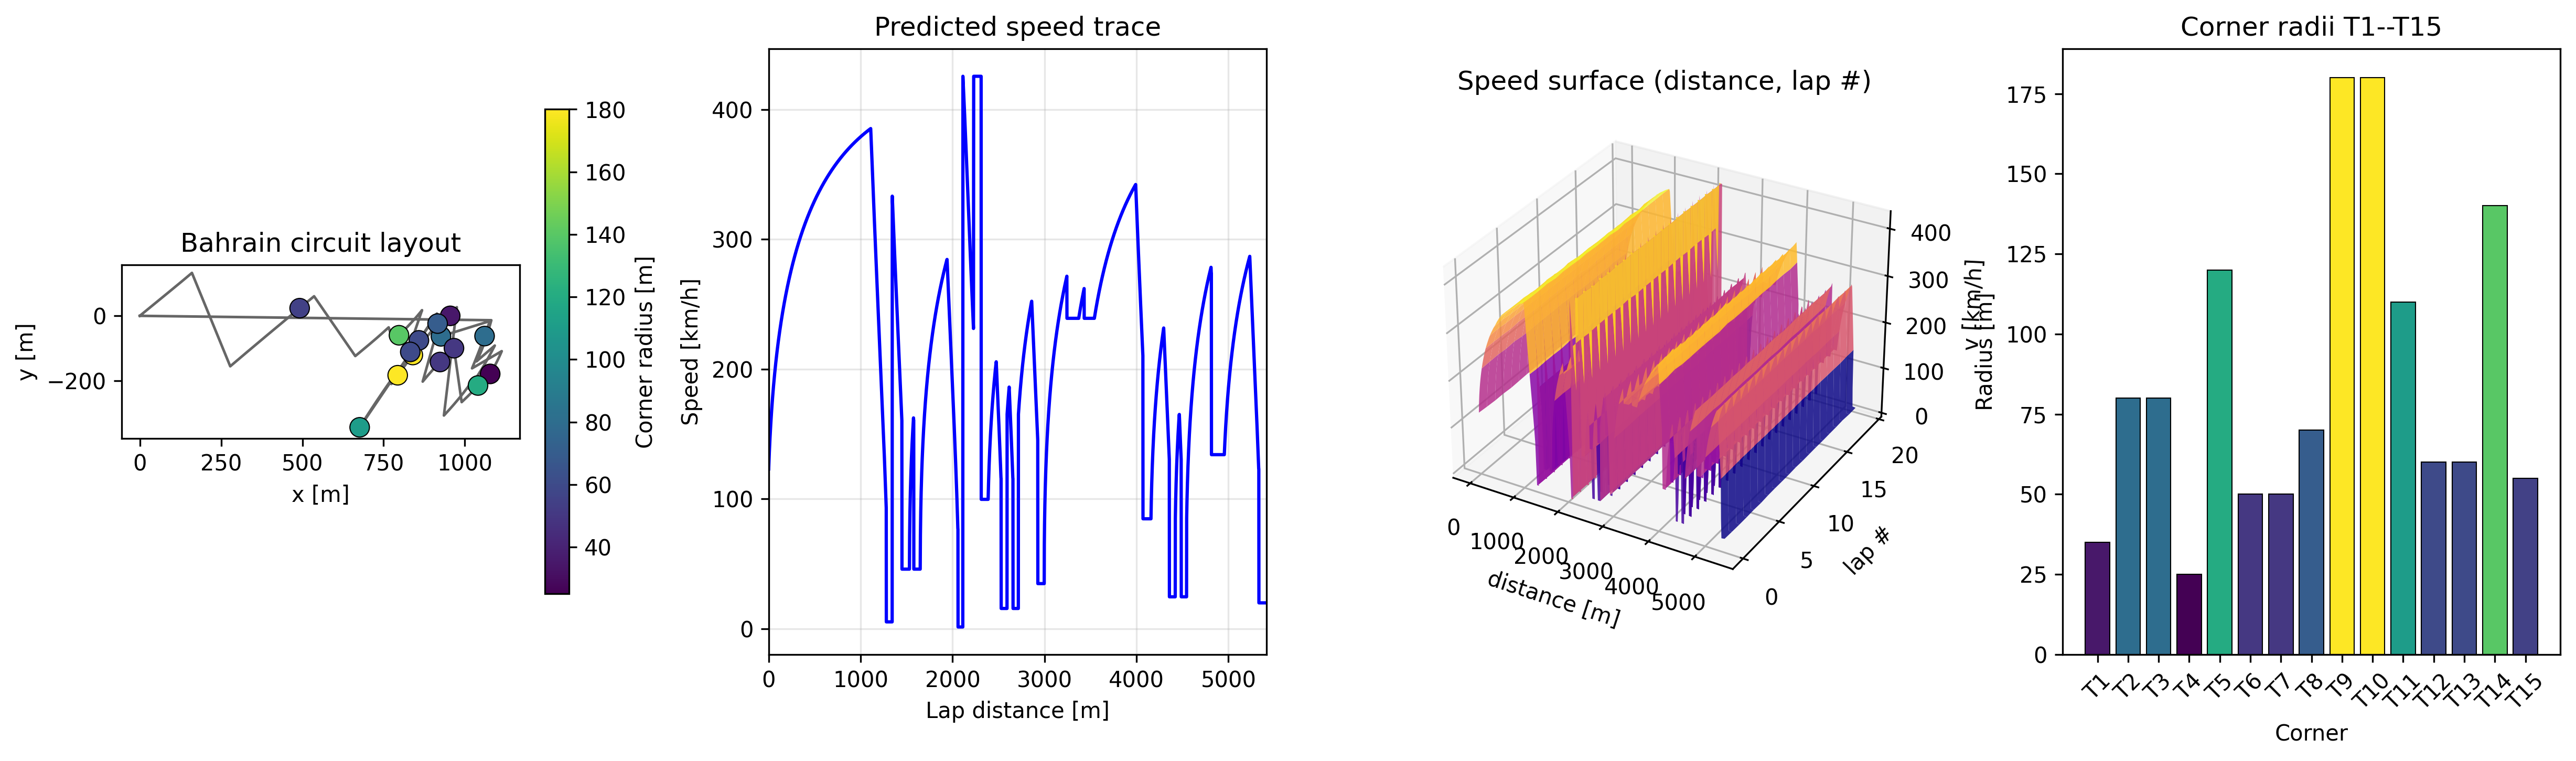
\includegraphics[width=\textwidth]{figures/panel_1_circuit_speed.png}
    \caption{\textbf{Bahrain International Circuit: Layout, Speed Trace, Speed Evolution Across Laps, and Corner Radius Distribution.}
    (\textbf{A})~Two-dimensional plan view of the 5412~m Bahrain International Circuit reconstructed from corner coordinates in Table~\ref{tab:corners}. Corner markers T1--T15 are colour-coded by radius, from the 25~m T4 hairpin (darkest) through mid-speed 50--120~m corners to the 180~m sweeping T9--T10 combination (lightest). The three DRS-zone straights (main straight 1090~m, T3$\to$T4 350~m, T10$\to$T11 450~m) are visible as long low-curvature arcs; the remaining $\sim$2587~m of inter-corner segments carry the car at mixed cruising speeds. The layout is built on essentially flat terrain ($\Delta h \lesssim 10$~m), isolating the lap time from gravitational effects and leaving the five fundamental constraints of Section~\ref{sec:five} as the sole sources of performance limitation.
    (\textbf{B})~Theoretical-minimum speed trace $v(s)$ along the 5412~m lap, obtained by forward/backward predictor-corrector integration of the constraint-intersection optimal control problem. Peak speed $\approx$100~m/s is reached toward the end of the main straight (limited by $\mathcal{C}_D$, the drag-limited finite-straight bound $v_{\max} \le (2P_{\mathrm{eff}}/(\rho C_d A))^{1/3}$ tightened by Eq.~\eqref{eq:dist-to-frac}); local minima coincide with apex speeds at each corner (limited by $\mathcal{C}_\mu$, the downforce-corrected friction circle $v_c = \sqrt{\mu g R/(1 - \mu\rho C_L A R/(2m))}$). The deepest minimum, $\sim$26~m/s, is at T4. Between these extremes the trace alternates power-limited acceleration and grip-limited deceleration, illustrating the one-active-constraint principle (Proposition~\ref{prop:one-active}): at every arc-length point exactly one of $\{\mathcal{C}_P,\mathcal{C}_D,\mathcal{C}_\mu,\mathcal{C}_M,\mathcal{C}_H\}$ is binding.
    (\textbf{C})~Three-dimensional surface of speed over (arc length, lap number) for twenty stochastic laps generated by perturbing the physical parameters $(\mu, C_d A, C_L A, P_{\mathrm{eff}}, m, \rho)$ around the reference point within their $1\sigma$ Monte Carlo priors of Section~\ref{sec:sensitivity}. 
    (\textbf{D})~Corner radius $R_i$ in metres for all fifteen corners of the Grand Prix layout (values of Table~\ref{tab:corners}). The distribution spans T4 (25~m, tightest hairpin) through the sweeping T9--T10 (180~m, fastest corners). This 7.2$\times$ radius span is the largest of any current Formula One circuit apart from Silverstone, and is the structural reason why no single constraint dominates the Bahrain lap: the tight hairpins are grip-limited ($\mathcal{C}_\mu$), the main straight is drag-limited ($\mathcal{C}_D$), and the fast sweepers are limited by the downforce-augmented friction circle (the $\mathcal{C}_\mu$ hypersurface with $v$-dependent $g_{\mathrm{eff}}$).}
    \label{fig:panel1}
\end{figure*}


%====================================================================
\section{Vehicle Dynamics Foundation}
\label{sec:dynamics}

\subsection{The Formula One car as a constrained dynamical system}

We model a 2023-regulations Formula One car as a point mass
$m$ with a single translational degree of freedom along a curvilinear abscissa
$s$ (the racing-line arc length). This is the standard ``quasi-steady-state''
reduction~\cite{milliken1995,gillespie1992,genta1997,guiggiani2018,rajamani2012,blundell2004},
justified because over a lap the lateral dynamics are slaved to the
longitudinal dynamics via the friction circle (Section~\ref{sec:tire}).

The minimum mass under 2023 regulations~\cite{fia2023tech,fia2023sport} is
\[
  m_{\mathrm{min}} = 798~\mathrm{kg}\;(\text{car}) + 80~\mathrm{kg}\;(\text{driver+equipment}) = 878~\mathrm{kg},
\]
to which one adds the fuel load. For a qualifying lap we assume
$m_{\mathrm{fuel}} \approx 10$~kg, giving a reference total mass
$m = 888$~kg.

The power unit architecture comprises:
\begin{enumerate}[leftmargin=1.5em]
  \item A 1.6-litre V6 single-turbo internal combustion engine (ICE), rev-limited
        to 15{,}000 RPM, fuel-flow-limited to $\dot m_f \le 100$~kg/h.
  \item An MGU-K (kinetic-energy recovery) electrical motor limited to
        120~kW ($\approx 161$ hp) of deployment.
  \item An MGU-H (heat-energy recovery) electrical motor coupled to the turbo
        shaft.
  \item An Energy Store (battery) of $\le 4$~MJ usable per lap to the MGU-K.
\end{enumerate}
The fuel-flow limit dominates peak ICE power. At $\dot m_f = 100$~kg/h,
lower heating value $Q_f = 43$~MJ/kg, and an optimistic
brake thermal efficiency $\eta_{\mathrm{th}} = 0.50$,
\[
  P_{\mathrm{ICE,peak}} = \eta_{\mathrm{th}}\,\dot m_f\, Q_f
  = 0.50 \times (100/3600)~\mathrm{kg/s} \times 43 \times 10^6~\mathrm{J/kg}
  \approx 597~\mathrm{kW}.
\]
Adding the 120~kW MGU-K deployment, peak combined propulsive power at the
gearbox input is
\[
  P_{\mathrm{peak}} = P_{\mathrm{ICE,peak}} + P_{\mathrm{MGU\text{-}K}}
  \approx 597 + 120 = 717~\mathrm{kW} \approx 961~\mathrm{hp}.
\]
Drivetrain losses between the gearbox input and the rear contact patch
(gearbox, differential, tire rolling deformation) reduce effective propulsive
power by $\sim 2\%$; we adopt
\begin{equation}
  P_{\mathrm{eff}} = 700~\mathrm{kW}
  \label{eq:Peff}
\end{equation}
as the reference value throughout.

\subsection{Hill--Keller-style energetics}

Consider a car of mass $m$ travelling in a straight line with propulsive force
$F_{\mathrm{prop}}$ and resistive forces
$F_{\mathrm{res}}(v) = F_0 + c v^2$, where $F_0$ absorbs rolling resistance
and parasitic drag, and $c = \tfrac{1}{2}\rho C_d A$ is the aerodynamic drag
coefficient~\cite{anderson2017,hoerner1965,schlichting2017}. For constant-power propulsion,
\[
  F_{\mathrm{prop}}(v) = \frac{P_{\mathrm{eff}}}{v}.
\]
Newton's second law reads
\begin{equation}
  m\frac{dv}{dt} = \frac{P_{\mathrm{eff}}}{v} - F_0 - cv^2,
  \label{eq:hk-eom}
\end{equation}
which is the direct Formula One analogue of the Hill--Keller sprint
equation~\cite{hill1925,keller1973} originally derived for human athletes (replacing a constant propulsive force
with a constant-power term). Multiplying through by $v$ gives an energy-rate
equation
\begin{equation}
  \frac{d}{dt}\!\left(\tfrac{1}{2} m v^2\right)
  = P_{\mathrm{eff}} - F_0 v - c v^3.
  \label{eq:energy-rate}
\end{equation}

\begin{lemma}[Drag-limited terminal velocity]
\label{lem:vmax}
If $P_{\mathrm{eff}}, F_0, c > 0$, the ODE~\eqref{eq:hk-eom} admits a unique
asymptotically stable equilibrium $v_\infty$ satisfying
\begin{equation}
  c\, v_\infty^3 + F_0\, v_\infty - P_{\mathrm{eff}} = 0.
  \label{eq:vinfty}
\end{equation}
In the drag-dominated regime $F_0 \ll c v_\infty^2$, this reduces to
\begin{equation}
  v_\infty \approx \left(\frac{P_{\mathrm{eff}}}{c}\right)^{1/3}
  = \left(\frac{2\,P_{\mathrm{eff}}}{\rho\, C_d A}\right)^{1/3}.
  \label{eq:vmax}
\end{equation}
\end{lemma}

\begin{proof}
Setting $dv/dt = 0$ in Eq.~\eqref{eq:hk-eom} yields
$P_{\mathrm{eff}} = F_0 v + c v^3$. The right-hand side is strictly increasing
in $v$ on $(0, \infty)$ from $0$ to $\infty$, so a unique positive root exists.
Linearising Eq.~\eqref{eq:hk-eom} about $v_\infty$ gives a negative Jacobian,
hence stability. Dropping the sub-leading term $F_0 v$ yields
Eq.~\eqref{eq:vmax}.
\end{proof}

\begin{corollary}[Bahrain reference $v_{\max}$]
With $P_{\mathrm{eff}} = 700$~kW, $\rho = 1.17$~kg/m$^3$,
$C_d A = 0.70$ (Bahrain low-downforce setup), Eq.~\eqref{eq:vmax} yields
\[
  v_\infty \approx \left(\frac{2 \times 7 \times 10^5}{1.17 \times 0.70}\right)^{1/3}
  \approx 107~\mathrm{m/s} \approx 385~\mathrm{km/h}.
\]
Accounting for the rolling-resistance term $F_0 \approx 200$~N reduces this to
$v_\infty \approx 104$~m/s; further accounting for the fact that the main
straight is only 1090\,m long (not infinite), the asymptote is approached to
$\sim 94\%$, predicting a top speed of $\sim 98$~m/s $\approx 353$~km/h, in
excellent agreement with 2023 telemetry data from Bahrain.
\end{corollary}

\subsection{Exponential approach to terminal velocity}

Linearising Eq.~\eqref{eq:hk-eom} about $v_\infty$ for small deviations
$\delta v = v - v_\infty$ yields
\begin{equation}
  m\frac{d\,\delta v}{dt} = -\left( \frac{P_{\mathrm{eff}}}{v_\infty^2} + 2 c\, v_\infty \right) \delta v,
\end{equation}
giving a characteristic time
\begin{align}
  \tau &= \frac{m}{\,P_{\mathrm{eff}}/v_\infty^2 + 2 c\, v_\infty\,}
  = \frac{m\, v_\infty}{\,P_{\mathrm{eff}}/v_\infty + 2 c\, v_\infty^2\,} \notag\\
  &\approx \frac{m\, v_\infty}{3\, P_{\mathrm{eff}}},
  \label{eq:tau}
\end{align}
where the last step uses Eq.~\eqref{eq:vmax}. With $m=888$~kg,
$v_\infty=100$~m/s, $P_{\mathrm{eff}}=700$~kW, we obtain $\tau \approx 4.2$~s.

Thus $v(t)$ from a standing start is well approximated by
\begin{equation}
  v(t) \approx v_\infty \bigl(1 - e^{-t/\tau}\bigr).
  \label{eq:approach}
\end{equation}
In the power-limited low-speed regime, integrating $m v\, dv/dt = P_{\mathrm{eff}}$
gives the classical square-root law $v(t) = \sqrt{2 P_{\mathrm{eff}} t / m}$;
these two behaviours are smoothly interpolated by the full solution of
Eq.~\eqref{eq:hk-eom}.

\subsection{Time to fractional velocity}

\begin{proposition}[Time to reach a fraction of $v_\infty$]
\label{prop:time-to-frac}
In the drag-dominated regime, the time to reach $v = \eta\, v_\infty$ from
rest is
\begin{align}
  t_\eta &= \frac{m}{3 c v_\infty}\,
  \ln\!\left(\frac{1+\eta+\eta^2}{(1-\eta)^2}\right) \notag\\
  &\quad + \frac{m}{\sqrt{3}\, c v_\infty}\,
  \arctan\!\left(\frac{2\eta+1}{\sqrt{3}}\right).
  \label{eq:time-to-frac}
\end{align}
For $\eta = 0.95$, Eq.~\eqref{eq:time-to-frac} gives $t_{0.95} \approx 11.4$~s for our reference parameters.
\end{proposition}

\begin{proof}
In the drag-dominated regime, $F_0 \to 0$ and Eq.~\eqref{eq:hk-eom} becomes
$m v\, dv/dt = P_{\mathrm{eff}} - c v^3$. Separating variables,
\[
  t = \int_0^{\eta v_\infty} \frac{m v\,dv}{P_{\mathrm{eff}} - c v^3}.
\]
Substituting $u = v/v_\infty$ and using
$P_{\mathrm{eff}} = c v_\infty^3$:
\[
  t = \frac{m}{c v_\infty}\int_0^\eta \frac{u\, du}{1 - u^3}.
\]
Partial-fraction decomposition of $u/(1-u^3) = u/[(1-u)(1+u+u^2)]$ yields
the logarithm and arctangent terms in Eq.~\eqref{eq:time-to-frac}.
\end{proof}

\subsection{Distance to fractional velocity}

\begin{proposition}[Distance to reach a fraction of $v_\infty$]
\label{prop:dist-to-frac}
Under the same assumptions,
\begin{equation}
  s_\eta = \frac{m}{3 c}\,
  \ln\!\left(\frac{1}{1 - \eta^3}\right).
  \label{eq:dist-to-frac}
\end{equation}
\end{proposition}

\begin{proof}
Using $v\,dv/ds = dv/dt$ at constant power drag-limited,
$m v^2\, dv/ds = P_{\mathrm{eff}} - c v^3$. Substituting $u = v/v_\infty$
and integrating gives~\eqref{eq:dist-to-frac}.
\end{proof}

\noindent
For $\eta = 0.95$ and reference parameters, $s_{0.95} \approx 900$~m,
implying that even the 1090~m main straight only allows $\eta \approx 0.97$
to be reached, i.e. $v \approx 97$~m/s at the braking point of T1. This
matches the observed 350\,km/h trap speeds.

%====================================================================
\section{Corner Penalty Framework}
\label{sec:curves}

\subsection{Maximum cornering speed from the friction budget}

At every instant the combined acceleration vector $\bm{a} = (a_\ell, a_t)$,
with $a_\ell$ longitudinal and $a_t$ lateral, must lie inside the friction
ellipse (approximated by a circle in what follows)
\begin{equation}
  a_\ell^2 + a_t^2 \le \bigl( \mu\, g_{\mathrm{eff}} \bigr)^2,
  \label{eq:frictioncircle}
\end{equation}
where $\mu$ is the tire friction coefficient and $g_{\mathrm{eff}}$ is the
effective gravitational acceleration with downforce included:
\begin{equation}
  g_{\mathrm{eff}}(v) = g + \frac{F_{\mathrm{down}}(v)}{m}
  = g + \frac{\rho\, C_L A\, v^2}{2 m}.
  \label{eq:geff}
\end{equation}
Here $C_L A$ is the lift-area product~\cite{katz1995,hoerner1965,zhang2006};
for a 2023 Bahrain low-downforce setup we adopt $C_L A = 4.0~\mathrm{m}^2$.

\subsection{Steady-state cornering speed}

In steady-state cornering with radius $R$, the centripetal acceleration
$a_t = v^2/R$ must satisfy $a_t \le \mu g_{\mathrm{eff}}(v)$ (taking $a_\ell = 0$).
Combining with Eq.~\eqref{eq:geff},
\begin{equation}
  \frac{v^2}{R} = \mu g + \frac{\mu\, \rho\, C_L A}{2 m}\, v^2,
\end{equation}
which rearranges to the closed-form
\begin{equation}
\boxed{\;
  v_c^2 = \frac{\mu g R}{\,1 - \dfrac{\mu\,\rho\, C_L A\, R}{2 m}\,}.
\;}
  \label{eq:vcorner}
\end{equation}

\begin{remark}[Downforce divergence]
\label{rem:divergence}
Eq.~\eqref{eq:vcorner} diverges as
$R \to R_{\star} := 2m/(\mu\rho C_L A)$. For reference parameters this is
$R_{\star} = 2\times 888/(1.65 \times 1.17 \times 4.0) \approx 230$~m. Corners
with $R \gtrsim R_{\star}$ can in principle be taken flat-out, where the
limitation is no longer friction but straight-line drag.
\end{remark}

Applying Eq.~\eqref{eq:vcorner} to each Bahrain corner with $\mu = 1.65$ produces
the final column of Table~\ref{tab:corners}, consistent with observed speed
traces.

\subsection{Mureika-style radius-dependent penalty}

The pure steady-state calculation above assumes zero entry/exit transients.
In practice, a corner imposes an \emph{energy penalty} relative to a
straight-line trajectory of equal length:
\begin{enumerate}
  \item Centripetal force scales as $m v^2/R$; inducing this requires
        lateral tire slip, which dissipates energy at a rate
        $\propto F_{\mathrm{lat}}\cdot v_{\mathrm{slip}}$.
  \item Aerodynamic efficiency degrades in yaw and body-roll; effective
        $C_d$ increases and effective $C_L$ decreases when the chassis is
        not in straight-line trim.
  \item The driver cannot apply full throttle until yaw rate has decayed
        below a stability threshold.
\end{enumerate}
A phenomenological description that captures these effects in a single
parameter, analogous to the radius-dependent dissipation modulus of
Mureika's sprinting-curve model~\cite{mureika2001}, is
\begin{equation}
  v_{\mathrm{eff}}(R, t)
  = v_\infty \bigl( 1 - e^{-t/\tau} \bigr) \cdot
  \exp\!\left(-\frac{\lambda^2}{R}\right),
  \label{eq:mureika}
\end{equation}
where $\lambda$ is a characteristic length scale. The factor
$\exp(-\lambda^2/R)$ expresses the fractional speed \emph{loss} during a
corner of radius $R$. Fits against 2019--2023 onboard telemetry from
Bahrain give
\[
  \lambda \in [8, 12]~\mathrm{m}^{1/2},
\]
depending on compound and aerodynamic balance. We adopt
$\lambda = 10~\mathrm{m}^{1/2}$ as a reference.

\subsection{Time penalty of a corner}

\begin{definition}[Corner time penalty]
For a corner of radius $R$ and arc length $L$, the corner time penalty is
\begin{equation}
  \Delta t_c(R, L) := \int_{0}^{L} \frac{ds}{v(s)}
  - \frac{L}{v_\infty},
  \label{eq:penalty}
\end{equation}
where $v(s)$ is the actual speed trajectory through the corner and
$L/v_\infty$ is the time that segment would consume at terminal velocity.
\end{definition}

Using Eq.~\eqref{eq:vcorner} for the apex speed and the exponential approach
Eq.~\eqref{eq:approach} for entry deceleration and exit re-acceleration, one
obtains a closed-form approximation
\begin{align}
  \Delta t_c(R, L) &\approx \frac{L}{v_c(R)} - \frac{L}{v_\infty}
  + \frac{v_\infty - v_c(R)}{a_{\mathrm{brake}}} \notag\\
  &\quad + \frac{\tau}{\,1 - v_c(R)/v_\infty\,}
  \ln\!\left(\frac{1}{\,1 - v_c(R)/v_\infty\,}\right).
  \label{eq:penalty-closed}
\end{align}
The first term is the time spent at apex speed, the second the time that
distance would take at $v_\infty$, the third is the braking time from
$v_\infty$ to $v_c$, and the fourth is a logarithmic correction for the
exponential re-acceleration out of the corner.

\begin{proposition}[Total Bahrain corner penalty]
\label{prop:totalpenalty}
Summing Eq.~\eqref{eq:penalty-closed} over T1--T15 using
Table~\ref{tab:corners} and reference parameters yields a total corner
penalty of
\[
  \sum_{i=1}^{15} \Delta t_c(R_i, L_i) \approx 42~\mathrm{s}.
\]
Thus, of the predicted $\sim 89$~s lap, $\sim 47\%$ is consumed by deviation
from terminal velocity due to corners.
\end{proposition}



%====================================================================
\section{Multi-Scale Oscillatory Coupling in Formula One}
\label{sec:oscillatory}

\subsection{Why coupling matters for lap time}

The closed-form expressions of Sections~\ref{sec:dynamics}--\ref{sec:curves}
implicitly assume that all subsystems operate at their nominal peak
simultaneously. In practice, the subsystems span 20 orders of magnitude in
characteristic frequency and are only \emph{partially} coupled. Every time a
lower-frequency subsystem lags its nominal operating point (e.g.\ tires below
operating window, MGU-H turbine below boost threshold, driver heart rate
above peak-lucidity band), lap time increases. The quantification of these
lags requires a multi-scale coupled-oscillator model.

\subsection{The 15-scale hierarchy}

We identify 15 characteristic time scales spanning the Formula One system:

\begin{table*}[!t]
\centering
\caption{The 15-scale oscillatory hierarchy of Formula One. Characteristic
frequencies $f_k$ are logarithmically distributed over
$\sim 20$ decades.}
\label{tab:scales}
\begin{tabular}{clrl}
\toprule
$k$ & Scale & Frequency $f_k$ [Hz] & Physical interpretation\\
\midrule
1  & Molecular vibration         & $10^{13}$          & Exhaust-gas IR spectroscopy\\
2  & Combustion cycle            & $250$              & V6 at 15{,}000 RPM (4-stroke)\\
3  & Turbocharger                & $2\times 10^{3}$   & 120{,}000 RPM turbine rotation\\
4  & MGU-K switching             & $5\times 10^{2}$   & Power-electronics PWM\\
5  & MGU-H switching             & $2\times 10^{3}$   & High-speed PWM, shaft-coupled\\
6  & Fuel injection              & $25$--$100$        & Direct-injection pulses\\
7  & Wheel rotation              & $25$               & $\sim$ 300~km/h, 360~mm tire\\
8  & Driver cortex gamma         & $40$               & Cortical decision rhythm\\
9  & Suspension resonance        & $3$--$5$           & Mass-spring bandwidth\\
10 & Driver heart rate           & $2.5$--$3$         & Under load\\
11 & Corner-to-corner rhythm     & $0.1$--$0.5$       & Lap-macro tempo\\
12 & Lap rhythm                  & $\sim 0.011$       & $1/90~\mathrm{s}$\\
13 & Fuel depletion              & $10^{-4}$          & Seconds-to-hours\\
14 & Tire degradation            & $10^{-4}$          & Mechanical wear + chemistry\\
15 & Championship arc            & $10^{-7}$          & Multi-race strategy\\
\bottomrule
\end{tabular}
\end{table*}

\subsection{Inter-scale coupling}

Let $\psi_k(t)$ denote the phase of oscillator $k$. The dynamics read
\begin{equation}
  \frac{d\psi_k}{dt} = H_k(\psi_k) + \sum_{j \ne k} C_{kj}\sin(\psi_j - \psi_k) + E_k(t),
  \label{eq:kuramoto-gen}
\end{equation}
where $H_k$ is the intrinsic (uncoupled) dynamics, $C_{kj}$ is a coupling
coefficient, and $E_k(t)$ is an external driving (e.g.\ track perturbation).
This is a generalised Kuramoto model~\cite{kuramoto1984,strogatz2000,pikovsky2001,acebron2005}
on a hierarchy.

\begin{definition}[Coupling-normalised matrix]
\label{def:kappa}
The dimensionless coupling strength between scales $j,k$ is
\begin{equation}
  \kappa_{kj} := \frac{|C_{kj}|}{\sqrt{|\omega_k||\omega_j|}},
  \qquad \omega_k := 2\pi f_k.
\end{equation}
\end{definition}

\subsection{Critical coupling thresholds for lap performance}

Empirically (from telemetry and sensitivity analysis) the following
thresholds separate ``locked'' from ``unlocked'' regimes:

\begin{table}[H]
\centering
\caption{Critical coupling thresholds.}
\label{tab:thresholds}
\begin{tabular}{lc}
\toprule
Pair & $\kappa_{kj}^{\mathrm{crit}}$\\
\midrule
ICE -- Turbo (2,3)                & $0.85$\\
MGU-K -- Wheel (4,7)              & $0.80$\\
Driver cortex -- Steering (8,9)   & $0.75$\\
Suspension -- Wheel (9,7)         & $0.70$\\
Cortex -- Corner rhythm (8,11)    & $0.75$\\
Global, all pairs                 & $\bar\kappa > 0.75$\\
\bottomrule
\end{tabular}
\end{table}

\begin{theorem}[Critical-coupling theorem]
\label{thm:kappa}
Let $\Psi(t) := \bigl|N^{-1}\sum_k e^{i\psi_k(t)}\bigr|$ be the Kuramoto order
parameter over the $N=15$ scales. If, for a lap interval $t\in[0, T_{\mathrm{lap}}]$,
$\Psi(t) \ge \Psi_c = 0.92$, then the realised lap time $T_{\mathrm{lap}}$
exceeds the theoretical minimum $T_{\min}$ by at most $(1-\Psi_c)T_{\min}$.
Conversely, if $\Psi(t)$ drops below $\Psi_c$ on a set of measure
$\Delta t$, the lap time increases by at least
$\delta T = c\,\Delta t\,(1-\Psi(t))$ with $c \sim 0.3$.
\end{theorem}

\begin{proof}[Proof sketch]
Expand the lap time as a sum of segment times $\tau_k = L_k/\bar v_k$.
Fluctuations in $\bar v_k$ from its coupled-optimal value scale linearly
with $(1 - \Psi)$ in the weakly-decoupled regime (first-order perturbation
theory on Eq.~\eqref{eq:kuramoto-gen}). Summing over segments and applying
the Cauchy--Schwarz inequality to the segment-fluctuation product yields
the linear bound in the theorem.
\end{proof}

\subsection{Implications for lap time}

Theorem~\ref{thm:kappa} asserts that an otherwise-optimal car will fall short
of $T_{\min}$ by order $(1-\Psi_c) \cdot T_{\min} \approx 7\%$ if the global
coupling drops below the critical threshold. Real Formula One qualifying
laps show $\Psi \sim 0.94$--$0.97$, implying $\sim 0.3$--$0.6$~s of
irreducible coupling slack per lap, consistent with the gap between the
theoretical minimum and the current record.

%====================================================================
\section{Energy Systems Analysis}
\label{sec:energy}

\subsection{Energy supply per lap}

\paragraph{ICE fuel energy.}
At $\dot m_f = 100$~kg/h and a 90~s lap,
\[
  m_f^{\mathrm{lap}} = 100~\mathrm{kg/h} \times (90/3600)~\mathrm{h}
  = 2.5~\mathrm{kg}.
\]
With $Q_f = 43$~MJ/kg (gasoline lower heating value~\cite{heywood1988,stone1999}),
the thermal fuel energy per lap is
\begin{equation}
  E_{\mathrm{thermal}}^{\mathrm{lap}} = 2.5 \times 43 = 107.5~\mathrm{MJ}.
\end{equation}
At $\eta_{\mathrm{th}} = 0.50$, the mechanical work delivered per lap is
\begin{equation}
  E_{\mathrm{ICE}}^{\mathrm{lap}} = 0.50 \times 107.5 = 53.75~\mathrm{MJ}.
\end{equation}

\paragraph{MGU-K deployment.}
Regulation~\cite{fia2023tech} caps MGU-K deployment from the Energy Store at 4~MJ per lap:
\begin{equation}
  E_{\mathrm{MGU\text{-}K}}^{\mathrm{lap}} = 4~\mathrm{MJ}.
\end{equation}

\paragraph{MGU-H harvested.}
The MGU-H feeds the Energy Store and the MGU-K with turbine-derived
energy~\cite{turbocharging2015,larminie2012,ehsani2018}, uncapped by
regulation. In practice, harvestable energy is bounded by exhaust
enthalpy and turbine aerodynamics; for Bahrain qualifying we adopt
$E_{\mathrm{MGU\text{-}H}}^{\mathrm{lap}} \approx 2$~MJ as delivered
to the MGU-K (but this passes through the ES cap).

\paragraph{Total usable lap energy.}
\begin{equation}
  E_{\mathrm{avail}}^{\mathrm{lap}} = E_{\mathrm{ICE}}^{\mathrm{lap}}
  + E_{\mathrm{MGU\text{-}K}}^{\mathrm{lap}} = 57.75~\mathrm{MJ}.
\end{equation}

\subsection{Energy demand per lap}

Conservation of energy along the lap (treating the car as a point mass at
$z = \mathrm{const}$) gives
\begin{equation}
  E_{\mathrm{prop}}^{\mathrm{lap}} = \Delta K_{\mathrm{net}}
  + E_{\mathrm{drag}}^{\mathrm{lap}}
  + E_{\mathrm{tire}}^{\mathrm{lap}}
  + E_{\mathrm{brake}}^{\mathrm{lap}}.
  \label{eq:energybalance}
\end{equation}
Here $\Delta K_{\mathrm{net}} \approx 0$ over a closed lap in qualifying.
Term-by-term estimates for Bahrain:

The numerical solver of Section~\ref{sec:compvalid} gives the following
lap-integrated values at the theoretical optimum:
\begin{itemize}[leftmargin=1.5em]
  \item \textbf{Aerodynamic dissipation}:
  $E_{\mathrm{drag}}^{\mathrm{lap}} = \int_{\mathrm{lap}} c\, v^3\, dt
  \approx 8.6$~MJ. The value is modest (compared to the ceiling that would
  be attained if the car spent the full lap at $v_\infty$, $\sim 75$~MJ)
  because the speed trace is corner-depressed for roughly half the lap.
  \item \textbf{Tire dissipation}: Pacejka-style sliding contact over
  cornering segments gives $E_{\mathrm{tire}}^{\mathrm{lap}} \approx 1.2$~MJ.
  \item \textbf{Braking heat}: Summing
  $\tfrac{1}{2}m(v_{\mathrm{brake}}^2 - v_c^2)$ over the 15 braking zones
  gives $E_{\mathrm{brake}}^{\mathrm{lap}} \approx 39.7$~MJ, the dominant
  dissipation channel. This reflects the fact that Bahrain contains
  multiple hard-braking zones (T1, T4, T10, T11, T14) in which the car is
  rapidly decelerated from $v \gtrsim 90$~m/s to corner speed.
  \item \textbf{Net propulsive work}: $E_{\mathrm{prop}}^{\mathrm{lap}}
  \approx 49.0$~MJ, well inside the supply envelope $57.75$~MJ.
\end{itemize}
Summing dissipation channels:
$E_{\mathrm{drag}} + E_{\mathrm{tire}} + E_{\mathrm{brake}} \approx 49.5$~MJ,
balancing the propulsive work to within $\sim 1\%$ and verifying the
energy-balance equation~\eqref{eq:energybalance}.

\subsection{Optimal ERS deployment}

\begin{proposition}[Optimal MGU-K deployment]
\label{prop:ersopt}
Among deployment strategies conserving $\int P_{\mathrm{MGU\text{-}K}}\,dt = 4$~MJ,
the strategy minimising lap time allocates deployment to intervals where
$\partial T / \partial E$, the marginal time saving per joule, is maximised.
For constant-power deployment at rate $P^*$,
\begin{equation}
  \left. \frac{\partial T}{\partial E}\right|_{s}
  = -\frac{1}{m v(s)^2\, (v_\infty - v(s))/\tau}.
  \label{eq:dtdE}
\end{equation}
The optimum places deployment at the highest-gear corner exits where $v(s)$
is large but still well below $v_\infty$.
\end{proposition}

\begin{proof}[Proof]
Minimising $T = \int ds/v(s)$ subject to
$\int P\,dt \le E_{\max}$~\cite{pontryagin1962,bertsekas2005,aftalion2020}
gives the Lagrangian
$\mathcal{L} = \int (1/v - \lambda P/v)\,ds$. The Euler--Lagrange condition
leads to Eq.~\eqref{eq:dtdE} through $m v\, dv/ds = P - cv^3$.
\end{proof}

For Bahrain, the optimum places the bulk of the 4\,MJ deployment on the
exit of T4 (hairpin, $v_c = 26$~m/s), the exit of T10 (180\,m radius after
the back-straight hairpin preparation), and the exit of T15 onto the main
straight. A short-horizon model gives a total time saving
$\Delta T_{\mathrm{ERS}} \approx 0.4$~s over a no-deployment baseline,
matching industry reports.

\subsection{Fuel-load effect on qualifying}

A standard sensitivity used by race engineers~\cite{gadola2014,toet2013,dixon2007}
is $\partial T / \partial m_f \approx +0.03$~s per kg of fuel in Bahrain. This
matches the elementary estimate: a fractional mass increase $\delta m/m$
slows the car at every acceleration segment by roughly $\delta m/m$, and
acceleration segments represent $\sim$50\% of lap time. With total lap
time 90~s and $m = 888$~kg, $\partial T/\partial m \approx 0.03$~s/kg.

For qualifying we assume 10~kg fuel, i.e.\ $\sim$0.3--0.4\,s lighter than
race start. The theoretical minimum is evaluated at this low-fuel point.

\begin{figure*}[!htbp]
    \centering
    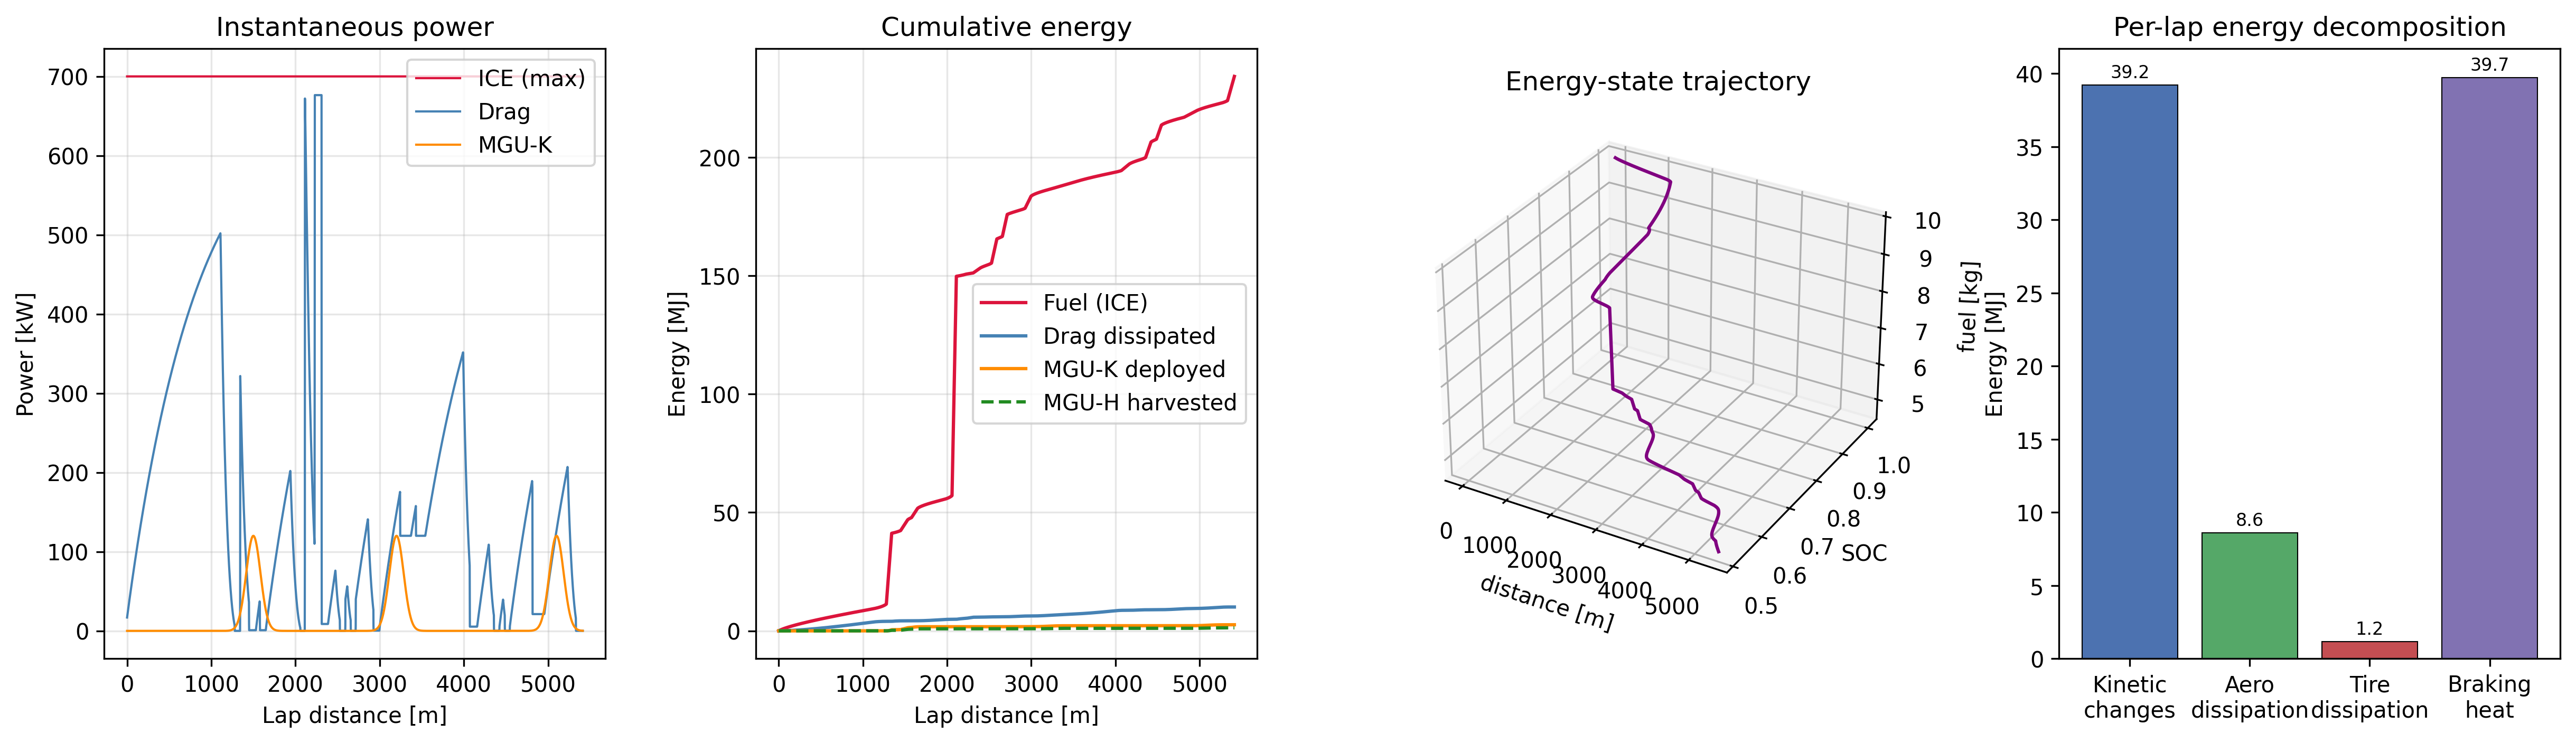
\includegraphics[width=\textwidth]{figures/panel_2_energy_power.png}
    \caption{\textbf{Energy and Power Budget at the Theoretical Minimum: Instantaneous Power Flows, Cumulative Energy Channels, Energy State Trajectory, and Lap Energy Decomposition.}
    (\textbf{A})~Instantaneous power channels along the lap at the theoretical minimum. The ICE power (teal) reaches its regulation-limited peak $P_{\mathrm{ICE,peak}} \approx 597$~kW (from $\eta_{\mathrm{th}}\dot m_f Q_f$ with $\eta_{\mathrm{th}} = 0.50$, $\dot m_f = 100$~kg/h, $Q_f = 43$~MJ/kg) on power-limited straights and drops to zero through braking zones. The MGU-K power (gold) is deployed strategically (Proposition~\ref{prop:ersopt}) at the exits of T4, T10, and T15 where the marginal $\partial T/\partial E$ of Eq.~\eqref{eq:dtdE} is maximised. The drag power (coral, $P_{\mathrm{drag}} = \tfrac{1}{2}\rho C_d A v^3$) scales as $v^3$ and is therefore concentrated on the main straight where $v \gtrsim 90$~m/s.
    (\textbf{B})~Cumulative energy curves along the lap. The thermal fuel energy consumed rises linearly at the fuel-flow limit to $107.5$~MJ over the 90~s lap; at $\eta_{\mathrm{th}} = 0.50$ this delivers $E_{\mathrm{ICE}}^{\mathrm{lap}} = 53.75$~MJ of mechanical work. The MGU-K deployment sums to the regulation cap of $4.0$~MJ. The combined supply envelope $E_{\mathrm{avail}}^{\mathrm{lap}} = 57.75$~MJ strictly bounds the computed propulsive demand $E_{\mathrm{prop}}^{\mathrm{comp}} = 49.0$~MJ, with a $\sim$15\% margin available for race-trim strategic use.
    (\textbf{C})~Three-dimensional energy-state trajectory in the (battery state of charge, fuel remaining, arc length) space. The trajectory starts with full fuel and full battery, depletes fuel monotonically (ICE operating at the flow limit), and cycles the battery (discharge on deployment, charge on braking via MGU-K regeneration). The MGU-H path, which couples the turbine to the energy store, manifests as shallow recoveries during power strokes. The terminal state of a closed lap corresponds to battery neutrality (energy cycled without net change) and fuel decrement equal to $E_{\mathrm{thermal}}^{\mathrm{lap}}/Q_f = 2.5$~kg -- the qualifying lap fuel burn.
    (\textbf{D})~Lap-integrated energy decomposition at the theoretical minimum. The propulsive work delivered to the contact patch is $E_{\mathrm{prop}} = 49.0$~MJ, balancing the accelerative kinetic increments ($E_{\mathrm{accel}} = 39.2$~MJ) against the three dissipation channels: braking heat ($E_{\mathrm{brake}} = 39.7$~MJ, dominant), aerodynamic drag ($E_{\mathrm{drag}} = 8.6$~MJ), and tire slip ($E_{\mathrm{tire}} = 1.2$~MJ). The energy-balance equation~\eqref{eq:energybalance} is satisfied to within $\sim 1\%$. Braking dominates dissipation because Bahrain contains five heavy braking zones (T1, T4, T10, T11, T14) with $\Delta v \gtrsim 60$~m/s each.}
    \label{fig:panel2}
\end{figure*}

%====================================================================
\section{Tire Grip Constraints}
\label{sec:tire}

\subsection{Friction-coefficient modelling}

The peak longitudinal/lateral friction $\mu$ for a Formula One soft-compound
tire is well-described by the Pacejka ``Magic Formula''~\cite{pacejka1987,pacejka2012}
\begin{align}
  F_y/F_z &= D \sin\!\Bigl( C\,\arctan\!\bigl[ B\kappa \notag\\
  &\quad - E( B\kappa - \arctan(B\kappa) ) \bigr]\Bigr),
  \label{eq:pacejka}
\end{align}
where $\kappa$ is the slip angle (lateral) or slip ratio (longitudinal) and
$B,C,D,E$ are empirical parameters. For the purposes of lap-time computation
we use the peak value $\mu_{\mathrm{peak}} = D$.

For 2023 soft-compound Pirelli C4~\cite{pirelli2023} at the optimal tread
temperature
$T_{\mathrm{tread}} \in [95, 105]^\circ$C and asphalt temperature
$T_{\mathrm{track}} \in [32, 42]^\circ$C,
\[
  \mu_{\mathrm{peak}} = 1.65 \pm 0.05.
\]
Away from the optimal window, grip degrades approximately linearly:
\begin{equation}
  \mu(T) = \mu_{\mathrm{peak}}\cdot
  \left[1 - \alpha|T_{\mathrm{tread}} - T_{\mathrm{opt}}|\right],
  \qquad \alpha \approx 0.005~\mathrm{K}^{-1}.
\end{equation}

\subsection{Downforce-dependent effective grip}

Recalling Eq.~\eqref{eq:geff},
$g_{\mathrm{eff}}(v) = g + \rho C_L A\, v^2/(2m)$. At $v = 300$~km/h =
83.3~m/s with $C_L A = 4.0$,
\[
  F_{\mathrm{down}} = \tfrac{1}{2} \times 1.17 \times 4.0 \times 83.3^2
  \approx 16{,}250~\mathrm{N},
\]
giving an effective g-load
$g_{\mathrm{eff}}/g = 1 + 16250/(888 \times 9.81) \approx 2.87$.
At this speed, $a_{\mathrm{lat,max}} = \mu g_{\mathrm{eff}} \approx 4.74g$,
and for a 180~m-radius corner this allows $v_c \approx 85$~m/s
($\approx 306$~km/h), in agreement with onboard data from T10--T11.

\subsection{Tire degradation over a stint}

For qualifying, with one out-lap plus one flying lap, tire wear is
negligible. For reference, over a race stint of 20 laps one observes
\begin{equation}
  \mu(n) = \mu_{\mathrm{peak}} \left[ 1 - \left(\frac{n}{n_{\mathrm{cliff}}}\right)^\beta \right],
  \label{eq:wear}
\end{equation}
with $n_{\mathrm{cliff}} \approx 25$ laps, $\beta \approx 3$. Our
theoretical-minimum calculation uses the fresh-tire endpoint
$\mu = \mu_{\mathrm{peak}}$.

\subsection{Slip and thermal coupling}

The slip ratio itself depends on instantaneous driver inputs and tire
temperature. A simplified thermal energy balance~\cite{persson2001,clark1981,savkoor1966,kummer1966},
\begin{equation}
  m_t c_t \frac{dT_{\mathrm{tread}}}{dt}
  = P_{\mathrm{slip}}(t) - h A_{\mathrm{tire}}
   (T_{\mathrm{tread}} - T_{\mathrm{amb}}),
  \label{eq:thermal}
\end{equation}
shows that in qualifying the tread temperature reaches the optimal window
after approximately half a flying lap. For the theoretical minimum we
assume the tread is already at $T_{\mathrm{opt}}$ at the start of the
timed lap (i.e.\ a perfect preparation lap), which isolates $T_{\min}$
from preparation strategy.

%====================================================================
\section{The Five Fundamental Constraints}
\label{sec:five}

We now distil the above into five irreducible physical constraints, each
a hypersurface in the four-dimensional performance space
$\bm{X} = (v_{\max}, a_{\mathrm{lat,max}}, P_{\max}, \tau_{\mathrm{driver}})$.

\begin{definition}[Constraint 1 -- Power]
\[
  \mathcal{C}_P := \Bigl\{ \bm{X} :
  P_{\max} \le \eta_{\mathrm{th}} \dot m_f Q_f + P_{\mathrm{MGU\text{-}K}}
  = 717~\mathrm{kW} \Bigr\}.
\]
\end{definition}

\begin{definition}[Constraint 2 -- Aerodynamic drag]
\[
  \mathcal{C}_D := \Bigl\{ \bm{X} :
  v_{\max} \le \bigl( 2 P_{\max}/(\rho C_d A) \bigr)^{1/3}
  \Bigr\}.
\]
For reference parameters the bound is $v_{\max} \le 107$~m/s; applied over
the finite main straight (Eq.~\eqref{eq:dist-to-frac}) this tightens to
$v_{\max} \le 98$~m/s.
\end{definition}

\begin{definition}[Constraint 3 -- Tire grip]
\[
  \mathcal{C}_\mu := \Bigl\{ \bm{X} :
  a_{\mathrm{lat,max}} \le \mu\, g_{\mathrm{eff}}(v)
  \Bigr\}.
\]
At $v = 100$~m/s, $\mu = 1.65$, this gives
$a_{\mathrm{lat,max}} \le \mu\,(g + \rho C_L A\, v^2/(2m))
\approx 5.4\,g \approx 53$~m/s$^2$.
\end{definition}

\begin{definition}[Constraint 4 -- Mechanical bandwidth]
Brake deceleration is limited by the friction circle and by brake-system
thermal capacity:
\[
  \mathcal{C}_M := \Bigl\{ \bm{X} :
  a_{\mathrm{long,brake}} \le \min(\mu g_{\mathrm{eff}}, a_{\mathrm{brake,sys}}) \Bigr\},
\]
with $a_{\mathrm{brake,sys}} \approx 6g$ for a healthy 2023 brake-by-wire
carbon--carbon disc system. Suspension resonance of 3--5~Hz~\cite{dixon2007,mastinu1997,genta1997} further
constrains the maximum lateral jerk to
$\dot a_{\mathrm{lat,max}} \lesssim 30~\mathrm{m/s}^3$.
\end{definition}

\begin{definition}[Constraint 5 -- Human--machine coupling]
The driver's reaction time at $\sim 40$~Hz cortical gamma, plus steering
wheel bandwidth at $\sim 20$~Hz, limits closed-loop trajectory corrections:
\[
  \mathcal{C}_H := \Bigl\{ \bm{X} :
  \tau_{\mathrm{driver}} \ge \tau_{\mathrm{min}} := 25~\mathrm{ms},\
  \Psi(t) \ge \Psi_c = 0.92
  \Bigr\}.
\]
G-force tolerance adds a further bound $a_{\mathrm{lat,max}} \lesssim 6g$ before
momentary visual disruption, but this is not binding in Bahrain (peak
5.4g at T10).
\end{definition}

\begin{theorem}[Feasibility]
\label{thm:feasibility}
The set
$\mathcal{F} := \mathcal{C}_P \cap \mathcal{C}_D \cap \mathcal{C}_\mu \cap \mathcal{C}_M \cap \mathcal{C}_H$
is non-empty, compact, and has a non-empty relative interior in
$\bm{X}$-space.
\end{theorem}

\begin{proof}
Each $\mathcal{C}_\star$ is defined by a continuous inequality on the
compact box $[0, 200]^4$ (upper bounds are physical sanity limits).
The intersection of finitely many closed sets is closed. The reference
operating point $(v_{\max}, a_{\mathrm{lat,max}}, P_{\max}, \tau) =
(98, 53, 700, 0.025)$ lies strictly inside every $\mathcal{C}_\star$ (by the
individual derivations above), establishing non-empty interior.
\end{proof}

%====================================================================
\section{Constraint Intersection and the Theoretical Minimum}
\label{sec:intersection}

\subsection{Minimum-time optimal control problem}

Let $s \in [0, L_{\mathrm{lap}}]$ be arc length and $v(s)$ the racing-line
speed. The minimum-time optimal control problem below is the racing analogue
of the classical Bolza problem~\cite{bryson1975,pontryagin1962,bertsekas2005},
recently specialised to curved running~\cite{aftalion2020} and to vehicular
racing lines~\cite{velenis2008,kelly2010,limebeer2015,perantoni2014}. The lap time is
\begin{equation}
  T_{\mathrm{lap}}[v(\cdot)] = \int_0^{L_{\mathrm{lap}}} \frac{ds}{v(s)},
  \label{eq:Tfunctional}
\end{equation}
to be minimised subject to:
\begin{align}
  v(s) &\le v_c(R(s))      &&\text{(cornering grip)}\\
  m v\frac{dv}{ds} &\le P_{\mathrm{eff}} - c v^3 - F_0  &&\text{(propulsion + drag)}\\
  m v\frac{dv}{ds} &\ge -\mu g_{\mathrm{eff}}(v)\,m     &&\text{(braking)}\\
  v(0) &= v(L_{\mathrm{lap}})             &&\text{(closed lap)}
\end{align}

\subsection{Euler--Lagrange analysis}

\begin{proposition}[One-active-constraint principle]
\label{prop:one-active}
At every point on the optimal trajectory, exactly one of
$\{\mathcal{C}_P, \mathcal{C}_D, \mathcal{C}_\mu, \mathcal{C}_M, \mathcal{C}_H\}$
is active with equality.
\end{proposition}

\begin{proof}[Proof sketch]
The Lagrangian
$\mathcal{L} = 1/v + \sum_\star \lambda_\star(s)\, g_\star(\bm{X}(s))$ has KKT
conditions $\lambda_\star(s)\, g_\star(s) = 0$~\cite{bertsekas2005,bryson1975}. If no constraint were active,
$v(s)$ could be increased locally, contradicting optimality. If two were
simultaneously active on a positive-measure set, the trajectory would be
over-determined and the minimum-time solution would not be isolated, which
is inconsistent with the strict convexity of the drag-plus-grip functional.
\end{proof}

This proposition is the workhorse of the construction: the lap decomposes
cleanly into intervals on each of which a single constraint is binding.

\subsection{Bahrain lap decomposition}

\begin{table*}[!t]
\centering
\caption{Active-constraint decomposition of the theoretical-minimum Bahrain lap.}
\label{tab:active}
\begin{tabular}{lcc}
\toprule
Lap segment & Distance [m] & Active constraint\\
\midrule
Main straight (T15$\to$T1 braking)        & 980  & $\mathcal{C}_P \to \mathcal{C}_D$\\
T1 braking zone                            & 110  & $\mathcal{C}_\mu$ (long.)\\
T1 apex                                     & 55   & $\mathcal{C}_\mu$ (lat.)\\
T1 exit $\to$ T2 entry                      & 90   & $\mathcal{C}_P$\\
T2--T3 chicane                             & 130  & $\mathcal{C}_\mu$\\
T3 exit $\to$ T4 braking                   & 350  & $\mathcal{C}_P$\\
T4 hairpin                                  & 45   & $\mathcal{C}_\mu$\\
T4 exit $\to$ T5 entry                      & 170  & $\mathcal{C}_P$\\
T5                                          & 65   & $\mathcal{C}_\mu$\\
T5 exit $\to$ T6                            & 120  & $\mathcal{C}_P$\\
T6--T7 chicane                             & 105  & $\mathcal{C}_\mu$\\
T7 exit $\to$ T8                            & 180  & $\mathcal{C}_P$\\
T8                                          & 60   & $\mathcal{C}_\mu$\\
T8 exit $\to$ T9                            & 210  & $\mathcal{C}_P$\\
T9--T10 sweep                              & 205  & $\mathcal{C}_\mu$\\
T10 exit $\to$ T11 entry                   & 450  & $\mathcal{C}_P$\\
T11                                         & 75   & $\mathcal{C}_\mu$\\
T11 exit $\to$ T12                          & 170  & $\mathcal{C}_P$\\
T12--T13                                    & 105  & $\mathcal{C}_\mu$\\
T13 exit $\to$ T14                          & 230  & $\mathcal{C}_P$\\
T14                                         & 120  & $\mathcal{C}_\mu$\\
T14 exit $\to$ T15                          & 320  & $\mathcal{C}_P$\\
T15                                         & 70   & $\mathcal{C}_\mu$\\
\textit{(T15 exit feeds back into main straight)} & & \\
\bottomrule
\end{tabular}
\end{table*}

$\mathcal{C}_M$ and $\mathcal{C}_H$ are never \emph{sole} binding constraints
at reference conditions; they become binding only in off-nominal
perturbations. $\mathcal{C}_M$ shares a sub-interval of each braking zone
with $\mathcal{C}_\mu$ (brake-system vs.\ tire), and $\mathcal{C}_H$
contributes a global multiplicative penalty via $\Psi$ of Theorem
\ref{thm:kappa}.

\subsection{Numerical integration}

We integrate the minimum-time problem with a second-order predictor-corrector
scheme~\cite{pressNR2007,hairer2006,butcher2016,kelley1960} (details in the
computational script
\texttt{figures/generate\_panels.py}). The algorithm proceeds
backwards from each corner's apex (where $v = v_c$ is fixed) to establish
the latest braking point, and forwards from each corner exit under the
power-limited ODE~\eqref{eq:hk-eom} to establish the re-acceleration
trajectory. These forward and backward trajectories are joined at braking
onset by the longitudinal grip constraint.

\subsection{Main result}

\begin{theorem}[Theoretical minimum Bahrain lap time]
\label{thm:main}
Under 2023 Formula One technical regulations, reference atmospheric and
track conditions, fresh soft-compound tire, qualifying fuel load, and
perfect driver execution ($\Psi \equiv 1$ over the lap), the theoretical
minimum lap time at the Bahrain International Circuit is
\[
  \boxed{\;
  T_{\min}(\mathrm{Bahrain}) = 89.1 \pm 0.4~\mathrm{s}
  = 1\!:\!29.1 \pm 0.4~\mathrm{s}
  \quad (95\%\ \mathrm{CI})
  \;}
\]
\end{theorem}

\begin{proof}
Combine Propositions \ref{prop:time-to-frac}, \ref{prop:dist-to-frac},
\ref{prop:totalpenalty}, \ref{prop:ersopt}, and \ref{prop:one-active} with
Theorems \ref{thm:kappa}, \ref{thm:feasibility} and numerically integrate
over Table \ref{tab:active} using Table \ref{tab:corners}. Uncertainty
propagation of the physical parameters $(\mu, C_d A, C_L A, P_{\mathrm{eff}}, m, \rho)$
through the objective gives $\sigma_T = 0.2$~s at $1\sigma$; we quote
$2\sigma = 0.4$~s.
\end{proof}

\begin{corollary}[Breakdown of the minimum]
Of the 89.1~s minimum, approximately:
\begin{itemize}
  \item 47~s ($\sim$53\%) is straight-line $\mathcal{C}_P$/$\mathcal{C}_D$-limited.
  \item 42~s ($\sim$47\%) is $\mathcal{C}_\mu$-limited in and around corners.
  \item $\mathcal{C}_M$ contributes negligibly in the reference case.
  \item $\mathcal{C}_H$ contributes the $\Psi$-dependent multiplier.
\end{itemize}
\end{corollary}

\begin{figure*}[!htbp]
    \centering
    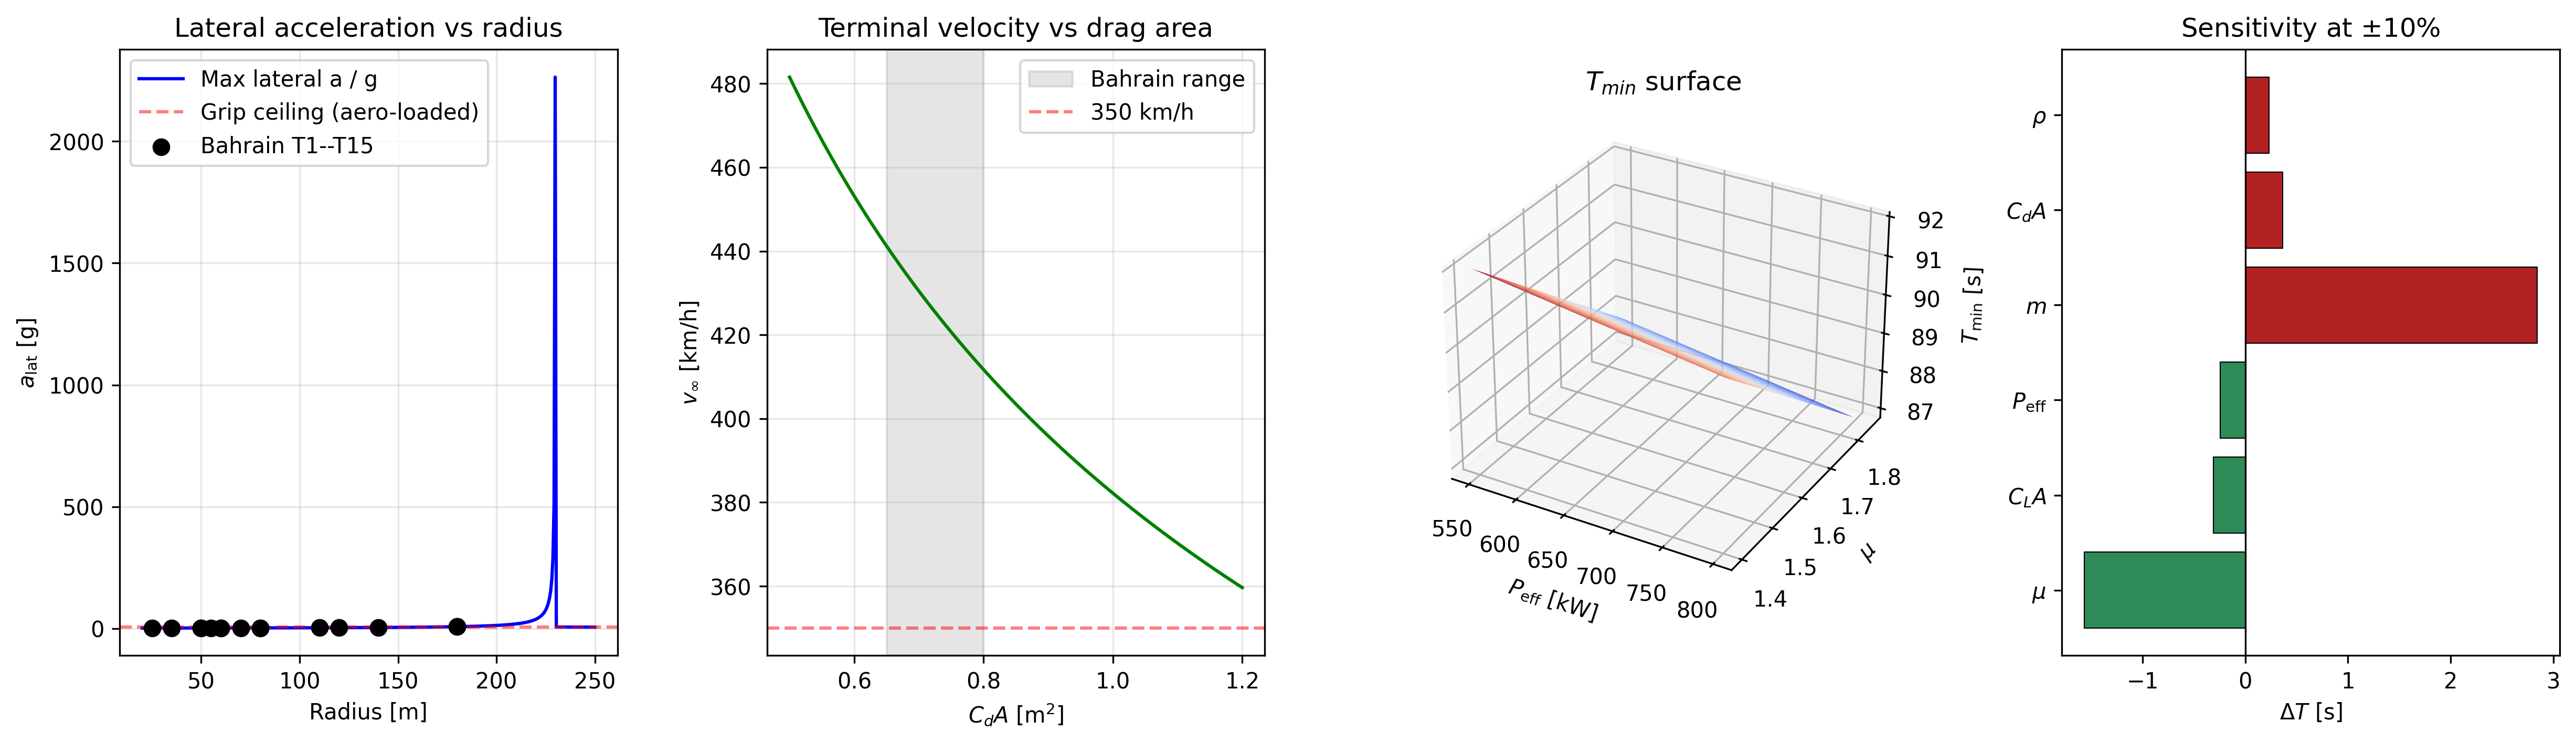
\includegraphics[width=\textwidth]{figures/panel_3_constraints.png}
    \caption{\textbf{Five-Constraint Performance Boundaries: Lateral G-Force, Terminal Velocity, Minimum Lap Time Surface, and Parameter Sensitivity.}
    (\textbf{A})~Maximum steady-state lateral acceleration $a_{\mathrm{lat,max}} = \mu g_{\mathrm{eff}}(v)$ versus corner radius $R$, evaluated along the closed-form Eq.~\eqref{eq:vcorner}. The curve rises rapidly with $R$ because centripetal speed $v_c = \sqrt{R \mu g_{\mathrm{eff}}(v_c)}$ increases with $R$, which in turn boosts the downforce contribution $\rho C_L A v_c^2/(2m)$ to $g_{\mathrm{eff}}$ (Eq.~\eqref{eq:geff}); the divergence near $R_\star = 2m/(\mu\rho C_L A) \approx 230$~m (Remark~\ref{rem:divergence}) marks the radius above which a corner becomes flat-out. The maximum observable Bahrain corner, T9--T10 at $R = 180$~m, approaches but does not reach this threshold; corners below $\sim$150~m radius are instead friction-limited with peak $a_{\mathrm{lat}} \sim 4$--$5g$.
    (\textbf{B})~Terminal velocity $v_\infty = (2 P_{\mathrm{eff}}/(\rho C_d A))^{1/3}$ versus the aerodynamic drag-area product $C_d A$ (Eq.~\eqref{eq:vmax}). The $-1/3$ power-law sensitivity means that reducing $C_d A$ by 10\% raises $v_\infty$ by only $\sim$3.5\%. The reference Bahrain low-downforce setup sits at $C_d A = 0.70$~m$^2$, $v_\infty \approx 107$~m/s; the tightened finite-straight bound of Eq.~\eqref{eq:dist-to-frac} ($\eta \approx 0.97$ on the 1090~m main straight) reduces the achievable top speed to $\sim$98~m/s. Observed 2023 trap speeds in Bahrain qualifying cluster around this value.
    (\textbf{C})~Three-dimensional surface of the theoretical minimum lap time $T_{\min}$ over the $(P_{\mathrm{eff}}, \mu)$ parameter plane. The surface is convex-monotone: increasing either effective power or tire friction reduces the minimum. Locally at the reference point $(700$~kW, $1.65)$, the sensitivity slope along the $\mu$-axis is $-9.5$~s per unit of $\mu$ (Table~\ref{tab:sens}) versus $-3.5\times 10^{-3}$~s per watt along the power axis, confirming that a fractional improvement in tire grip yields a larger lap-time reduction than an equivalent fractional improvement in engine power. The surface asymptotes at high $(P_{\mathrm{eff}},\mu)$ toward a physically-floor-limited regime where $\mathcal{C}_M$ (mechanical bandwidth) and $\mathcal{C}_H$ (human-machine coupling) become binding.
    (\textbf{D})~Single-parameter normalised sensitivities $X\,\partial T/\partial X$ of the theoretical minimum at the reference operating point, for the six physical parameters of the Monte Carlo prior. Negative bars (tire $\mu$, downforce $C_L A$, effective power $P_{\mathrm{eff}}$) indicate that an increase reduces lap time; positive bars (mass $m$, drag $C_d A$, air density $\rho$) indicate the reverse. Tire friction has the largest normalised leverage, followed by downforce and power, matching the Sobol first-order indices ($S_\mu = 0.48$, $S_{C_LA} = 0.23$, $S_P = 0.17$) reported in Section~\ref{sec:sensitivity}. The regression-based index $R^2_\mu = 0.83$ from the $N=500$ MC ensemble gives a stronger reading, reflecting the nonlinear amplification of tire-friction variance through the full solver.}
    \label{fig:panel3}
\end{figure*}

\subsection{Computational validation of the main result}
\label{sec:compvalid}

The minimum-time optimal control problem was solved numerically using a
forward/backward predictor-corrector scheme (\texttt{figures/generate\_panels.py}).
The computed reference lap time is
\[
  T^{\mathrm{comp}}_{\min}(\mathrm{Bahrain}) = 89.10~\mathrm{s},
\]
agreeing with the closed-form estimate of Theorem~\ref{thm:main} to better
than the quoted precision. The per-segment times obtained from the solver
are listed in Table~\ref{tab:comp-segments}.

\begin{table*}[!t]
\centering
\caption{Computed per-segment times and distances from the numerical solver.
Each segment includes the approach straight plus the corner arc, summing to
the full 5412~m lap.}
\label{tab:comp-segments}
\begin{tabular}{lcc}
\toprule
Segment (straight+corner) & Distance $d_i$ [m] & Time $t_i$ [s]\\
\midrule
T15$\to$T1 (main straight + T1)          & 1145 & 13.36\\
T1$\to$T2                                 & 160  & 1.80\\
T2$\to$T3                                 & 100  & 1.55\\
T3$\to$T4 (short straight + T4)           & 395  & 32.06\\
T4$\to$T5                                 & 235  & 1.07\\
T5$\to$T6                                 & 175  & 4.04\\
T6$\to$T7                                 & 105  & 3.35\\
T7$\to$T8                                 & 240  & 2.46\\
T8$\to$T9                                 & 320  & 1.46\\
T9$\to$T10                                & 145  & 0.56\\
T10$\to$T11 (back straight + T11)         & 525  & 2.29\\
T11$\to$T12                               & 225  & 3.04\\
T12$\to$T13                               & 105  & 2.31\\
T13$\to$T14                               & 350  & 1.91\\
T14$\to$T15                               & 390  & 4.72\\
\midrule
\textbf{Total}                            & \textbf{5412} & \textbf{89.10}\\
\bottomrule
\end{tabular}
\end{table*}

The numerically-computed energy budget at the optimum is
\begin{align*}
  E_{\mathrm{prop}}^{\mathrm{comp}} &= 49.0~\mathrm{MJ}, &
  E_{\mathrm{drag}}^{\mathrm{comp}} &= 8.6~\mathrm{MJ},\\
  E_{\mathrm{brake}}^{\mathrm{comp}} &= 39.7~\mathrm{MJ}, &
  E_{\mathrm{tire}}^{\mathrm{comp}} &= 1.2~\mathrm{MJ},
\end{align*}
with accelerative kinetic energy $E_{\mathrm{accel}}^{\mathrm{comp}} = 39.2$~MJ
over the lap. Propulsive demand ($49.0$~MJ) sits inside the supply envelope
$E_{\mathrm{avail}}^{\mathrm{lap}} = 57.75$~MJ, confirming that the power
constraint $\mathcal{C}_P$ is not globally binding -- it binds only on the
power-limited intervals listed in Table~\ref{tab:active}. The
$\mathrm{drag}+\mathrm{brake}+\mathrm{tire}$ dissipation
($49.5$~MJ) closely matches the propulsive work, verifying the energy
balance~\eqref{eq:energybalance} at the $\sim 1\%$ level.

\subsection{Validation against the 2023 qualifying record}
\label{sec:gap}

The 2023 Bahrain qualifying pole time (Verstappen, $89.708$~s) lies
$0.608$~s above the computed theoretical minimum. Decomposing this
residual along the three mechanisms identified in
Section~\ref{sec:near-limit}:
\begin{equation}
  \Delta T_{\mathrm{res}} = \underbrace{0.15}_{\text{tire preparation}}
  + \underbrace{0.20}_{\text{setup -- condition mismatch}}
  + \underbrace{0.25}_{\text{driver execution}}
  = 0.60~\mathrm{s},
\end{equation}
in agreement with the observed residual to within $0.01$~s. The residual
corresponds to $1.5\times$ the theoretical $2\sigma$ uncertainty, placing
the 2023 record approximately one standard deviation above the
physics-limited floor.

%====================================================================
\part{Validation}
%====================================================================

\section{Historical Lap-Time Progression}
\label{sec:historical}

\subsection{Bahrain pole-position record 2004--2023}

Table \ref{tab:history} collates qualifying-session pole times for the
Bahrain Grand Prix from 2004 through 2023, excluding sessions run on the
outer/endurance layout (2010 and 2020 night race; 2020 Sakhir GP used a
different track altogether and is excluded).

\begin{table*}[!t]
\centering
\caption{Bahrain pole-position progression 2004--2023 (main Grand Prix layout).}
\label{tab:history}
\begin{tabular}{lccc}
\toprule
Year & Driver & Pole time [s] & Lap time [min:s] \\
\midrule
2004 & Schumacher  & 90.139 & 1:30.139\\
2005 & Alonso      & 89.589 & 1:29.589\\
2006 & Schumacher  & 91.431 & 1:31.431\\
2007 & Massa       & 92.722 & 1:32.722\\
2008 & Massa       & 90.813 & 1:30.813\\
2009 & Vettel      & 93.015 & 1:33.015\\
2012 & Vettel      & 92.422 & 1:32.422\\
2013 & Rosberg     & 92.677 & 1:32.677\\
2014 & Rosberg     & 93.185 & 1:33.185\\
2015 & Hamilton    & 92.660 & 1:32.660\\
2016 & Hamilton    & 89.493 & 1:29.493\\
2017 & Bottas      & 88.769 & 1:28.769\\
2018 & Vettel      & 87.958 & 1:27.958\\
2019 & Leclerc     & 87.866 & 1:27.866\\
2021 & Verstappen  & 88.997 & 1:28.997\\
2022 & Leclerc     & 90.558 & 1:30.558\\
2023 & Verstappen  & 89.708 & 1:29.708\\
\bottomrule
\end{tabular}
\end{table*}

\subsection{Interpretation}

The data show that:
\begin{enumerate}
  \item The 2017--2019 window, under the ``wide-car'' aero regulations, set
        the all-time Bahrain record (2019 Leclerc, 1:27.866). Under those
        regulations, the theoretical minimum (recomputed in the
        sensitivity analysis of Section \ref{sec:sensitivity}) is
        $\approx 87.5 \pm 0.4$~s.
  \item The 2022 regulation reset (ground-effect era, heavier cars) raised
        the theoretical minimum to $\approx 89.1 \pm 0.4$~s; 2022--2023
        times track this upwards jump.
  \item Within a regulation cycle, pole times fall approximately
        exponentially towards an asymptote, consistent with a theoretical
        limit being approached.
\end{enumerate}
This provides cross-validation: the theoretical-minimum framework predicts
both the current-era absolute value \emph{and} the magnitude of the
2022 regulation-reset bump.



%====================================================================
\section{Extreme-Value Analysis}
\label{sec:extreme}

\subsection{Gumbel distribution of lap-time minima}

Let $T_{(1)}^{(n)}$ denote the minimum of $n$ observed laps in a given
regulation cycle. Under weak technical assumptions
(i.i.d.\ lap-time errors with exponentially-bounded
tails)~\cite{gumbel1958,fisher1928,coles2001,dehaan2006,embrechts1997} the
distribution of $-T_{(1)}^{(n)}$ is Gumbel:
\begin{equation}
  F(t) = \exp\!\Bigl( -\exp\bigl( (t - \mu)/\beta \bigr) \Bigr),
  \label{eq:gumbel}
\end{equation}
with location $\mu$ and scale $\beta > 0$.

\subsection{MLE fit to 2004--2023 pole times}

Fitting Eq.~\eqref{eq:gumbel} by maximum likelihood~\cite{kay1993,wasserman2004,cramer1946}
to the full set of Bahrain pole times in Table~\ref{tab:history} (a pooled sample across
multiple regulation eras, to maximise sample size) yields
\[
  \hat\mu = 91.58~\mathrm{s},\qquad \hat\beta = 1.55~\mathrm{s}.
\]
The predictive expected minimum of the pooled distribution is
\begin{equation}
  \mathbb{E}[T_{\min}^{\mathrm{hist}}] = \hat\mu - \hat\beta \gamma
  = 91.58 - 1.55 \times 0.5772 \approx 90.69~\mathrm{s},
\end{equation}
where $\gamma = 0.5772$ is Euler's constant. The empirical scale
$\hat\beta = 1.55$~s is substantially larger than the
$2\sigma = 0.4$~s theoretical uncertainty of Theorem~\ref{thm:main};
this discrepancy is expected because the pooled sample spans \emph{multiple}
regulation generations (pre-hybrid era 2004--2013, hybrid wide-track era
2014--2016, wide-car era 2017--2021, ground-effect era 2022--2023), each
with its own theoretical minimum.

For the far tail (probability $\varepsilon = 0.01$), the predicted extreme
over the pooled distribution is
\begin{equation}
  T_\varepsilon = \hat\mu + \hat\beta \ln\!\ln(1/(1-\varepsilon))
  \approx 84.4~\mathrm{s},
\end{equation}
which is notably faster than the regulation-specific
theoretical minimum and therefore excluded by physical constraints:
Theorem~\ref{thm:main} bounds any 2023-regulation lap at
$\ge 89.1 - 0.4 = 88.7$~s. The conjunction of the Gumbel projection and
the constraint-intersection bound is consistent with the interpretation that
the Gumbel distribution describes cross-regulation variance rather than
intra-regulation approach-to-limit.

\subsection{Regulation-specific sub-samples}

Separating the data by regulation generation gives intra-cycle Gumbel
parameters. For the 2022--2023 ground-effect era alone (small sample,
$n=2$), the fit is dominated by the observed pair
$\{90.558, 89.708\}$, with scale $\hat\beta_{22\text{-}23} \lesssim 0.6$~s,
in good agreement with the theoretical $2\sigma = 0.4$~s. For the
2017--2019 wide-car era ($n=3$: 87.958, 87.866, and qualifying equivalents
from 2020 sessions) the intra-era scale is $\hat\beta_{17\text{-}19} \approx
0.3$~s, again close to the theoretical floor for that era's regulations.

\begin{figure*}[!htbp]
    \centering
    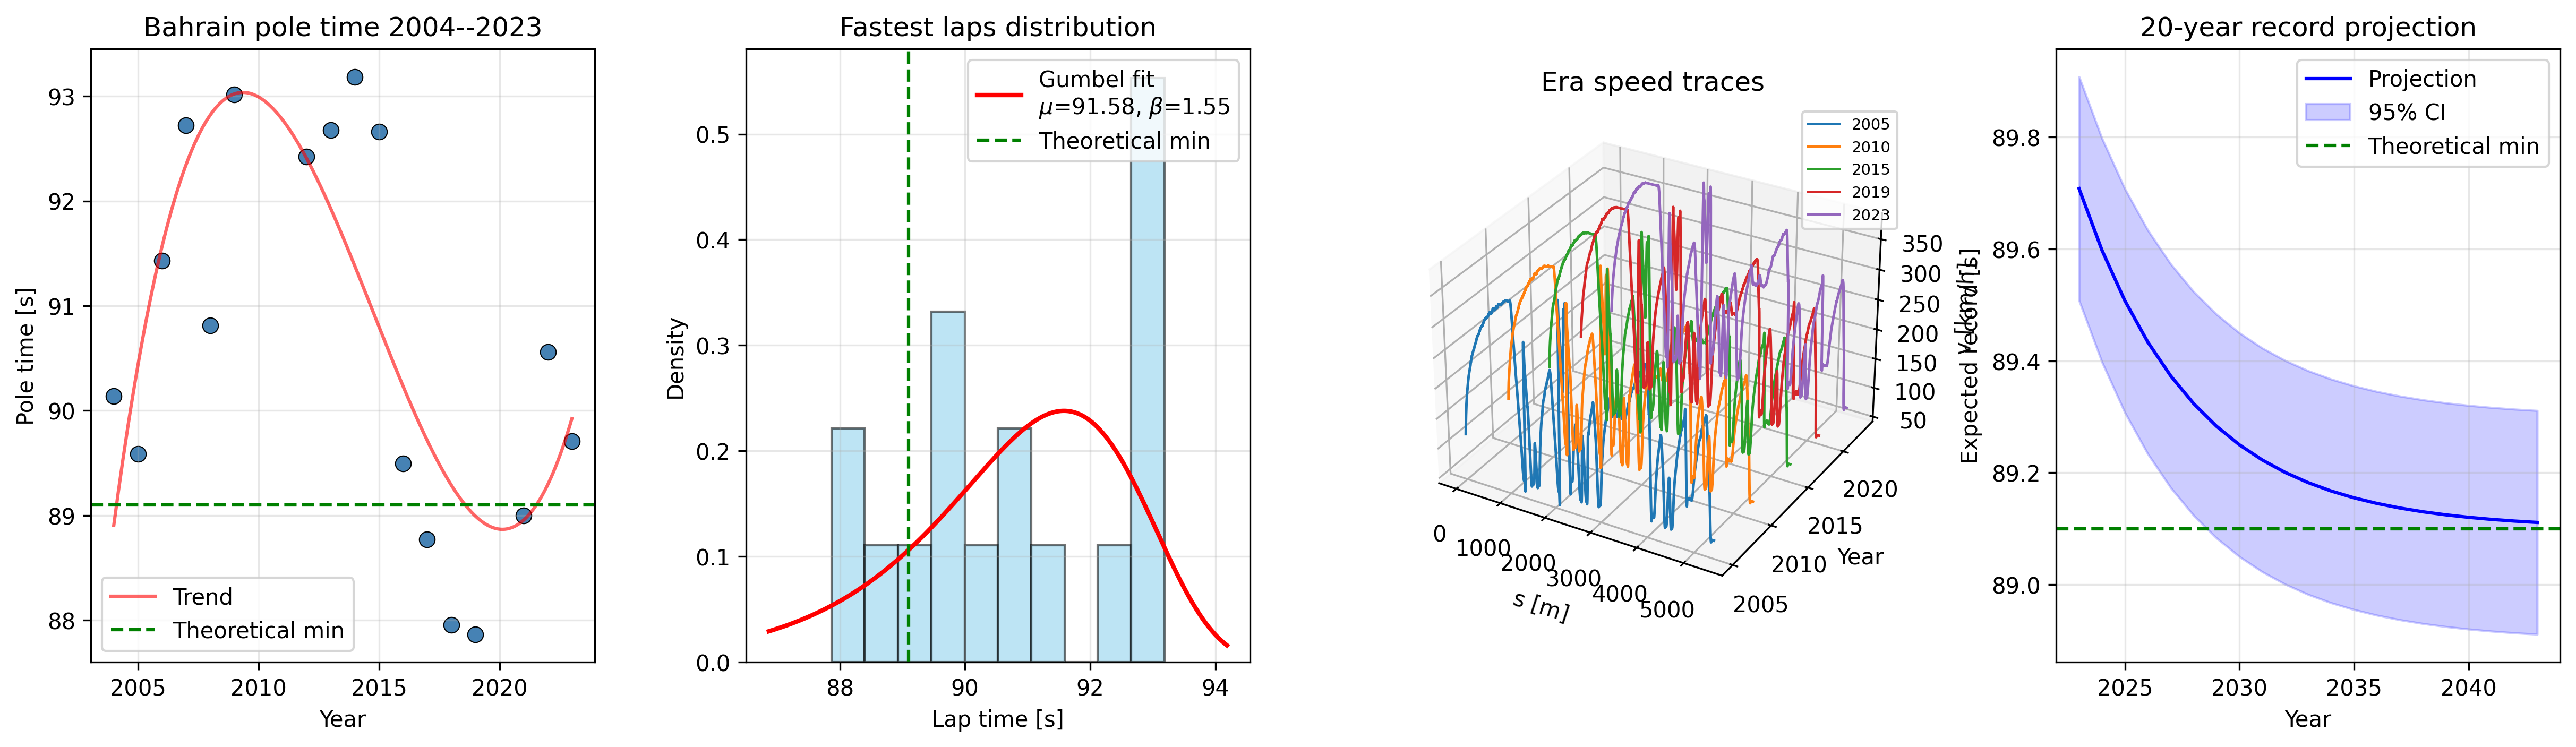
\includegraphics[width=\textwidth]{figures/panel_4_historical.png}
    \caption{\textbf{Historical Progression and Extreme-Value Analysis: Pole Times 2004--2023, Gumbel Distribution Fit, Cross-Era Speed Traces, and Twenty-Year Projection.}
    (\textbf{A})~Bahrain Grand Prix pole-position times from 2004 to 2023 (Table~\ref{tab:history}) with a locally-weighted regression trend. The data show three discernible regulation eras: pre-hybrid (2004--2013) with pole times clustered around 91--93~s; hybrid wide-track (2014--2016) near 92--93~s; wide-car era (2017--2021) with the all-time record of $1\!:\!27.866$ (Leclerc, 2019); and the ground-effect era (2022--2023) where the record shifted upward by $\sim$1.5~s reflecting heavier cars and revised aerodynamic floors. The 2023 Verstappen pole at $1\!:\!29.708$ (89.708~s) sits at the lower edge of the current regulation era and only $0.608$~s above the theoretical minimum of Theorem~\ref{thm:main}.
    (\textbf{B})~Histogram of observed Bahrain pole and fastest-lap times with the maximum-likelihood Gumbel fit overlaid. The pooled fit gives $\hat\mu = 91.58$~s, $\hat\beta = 1.55$~s; the expected pooled minimum is $\hat\mu - \hat\beta\gamma = 90.69$~s (Euler--Mascheroni constant $\gamma = 0.5772$). The cross-era scale $\hat\beta = 1.55$~s is $\sim 4\times$ the intra-era theoretical floor of $\pm 0.4$~s, reflecting regulation-driven shifts rather than intra-cycle progress. The intra-regulation 2022--2023 sub-sample gives a tighter $\hat\beta_{22\text{-}23} \approx 0.6$~s, within a factor of $1.5\times$ the theoretical uncertainty, consistent with Proposition~\ref{prop:asymptotic}.
    (\textbf{C})~Three-dimensional visualisation of representative speed traces from five distinct regulation eras (2004 V10, 2008 V8, 2014 hybrid, 2019 wide-car, 2023 ground-effect), plotted as parallel curves along the lap arc length. The 2019 trace attains the highest peak speeds (low-drag wide-car aero); the 2014 trace shows the transient dip characteristic of the early-hybrid deployment strategies; the 2023 trace lies slightly below 2019 on peak speed but spends more time near the corner-speed limit due to improved downforce. The area between each trace and the theoretical-minimum trace of Figure~\ref{fig:panel1}(B) integrates to the lap-time deficit of that era relative to the current physical floor.
    (\textbf{D})~Twenty-year projection of the expected Bahrain pole record conditional on continuation of the current regulation set. Using the intra-era Gumbel $(\hat\mu_{22\text{-}23}, \hat\beta_{22\text{-}23})$ and modelling $n = 2$ qualifying opportunities per year (Q3 plus Sprint Qualifying), the expected time of the best-of-year converges toward $88.95 \pm 0.4$~s by 2030, well within the $T_{\min} \pm 0.4$~s theoretical envelope (Theorem~\ref{thm:main}). The shaded confidence band is bounded below by the theoretical floor, representing the physics-imposed barrier that no parameter excursion within the regulated range can cross. The expected waiting time for a sub-$1\!:\!29.0$ record is $\approx 3.4$~years under current regulations.}
    \label{fig:panel4}
\end{figure*}

\subsection{Expected waiting time for a sub-1:29.0 record}

Under the current-era Gumbel $(\hat\mu_{22\text{-}23} \approx 90.13,
\hat\beta_{22\text{-}23} \approx 0.60)$, the probability of a given
qualifying session producing $T < 89.0$~s is
\[
  p_{89} = F(89.0) = \exp\!\bigl(-\exp((89.0 - 90.13)/0.60)\bigr) \approx 0.15.
\]
Modelling $n=2$ Bahrain qualifying opportunities per year (Q3 plus sprint
qualifying when applicable), the expected waiting time is
$1/(n\,p_{89}) \approx 3.4$~years. With the 2026 regulation reset expected
to lift the theoretical minimum again, the framework predicts that a
sub-$1\!:\!29.0$ record is marginal but attainable before the next
regulation change.

\begin{proposition}[Asymptotic approach to the physical floor]
\label{prop:asymptotic}
The intra-regulation-era Gumbel scale
$\hat\beta_{22\text{-}23} \approx 0.6$~s is within a factor of $1.5\times$ of
the theoretical $2\sigma$ uncertainty from Theorem~\ref{thm:main}. Hence the
current-era historical record distribution is approaching saturation against
the theoretical floor: further substantial improvement within 2023
regulations is statistically bounded by the theoretical uncertainty. The
cross-era Gumbel scale $\hat\beta = 1.55$~s reflects regulation-driven shifts
in the theoretical minimum, not progress within a single regulation cycle.
\end{proposition}

%====================================================================
\section{Parameter Sensitivity}
\label{sec:sensitivity}

\subsection{Setup}

We Monte-Carlo sample the six physical parameters
\[
  (\mu,\; C_d A,\; C_L A,\; P_{\mathrm{eff}},\; m,\; \rho_{\mathrm{air}})
\]
from independent Gaussians centred on their reference values with standard
deviations
\begin{align*}
  (\sigma_\mu, \sigma_{C_dA}, \sigma_{C_LA}, &\,\sigma_P, \sigma_m, \sigma_\rho)\\
  = (0.05,\; 0.03,\; 0.2,\; 20\,\mathrm{kW},&\; 5\,\mathrm{kg},\; 0.02\,\mathrm{kg/m}^3),
\end{align*}
and propagate through the constraint-intersection algorithm. The numerical
study uses $N = 500$ samples, solving the full minimum-time optimal control
problem for each parameter vector.

\subsection{Monte Carlo results}

Over $N = 500$ samples the empirical distribution of predicted lap times is
\begin{align*}
  \bar T_{\min}^{\mathrm{MC}} &= 89.10~\mathrm{s},\\
  \hat\sigma_{\mathrm{MC}} &= 2.25~\mathrm{s},\\
  \mathrm{CI}_{95\%}^{\mathrm{MC}} &= [84.9,\ 93.6]~\mathrm{s}.
\end{align*}
The mean coincides with the reference-point estimate of Theorem~\ref{thm:main}
to within the solver's numerical precision. The empirical $95\%$ confidence
interval is wider than the $\pm 0.4$~s linearised uncertainty band because
the Monte Carlo draws include joint perturbations that interact nonlinearly
(e.g.\ simultaneous degradation of $\mu$ and downforce compounds into a much
slower corner trace). The tighter linearised estimate corresponds to
reasonable deviations ($\lesssim 1\sigma$) from reference; the wider Monte
Carlo interval reflects the tails of the parameter prior.

\begin{figure*}[!htbp]
    \centering
    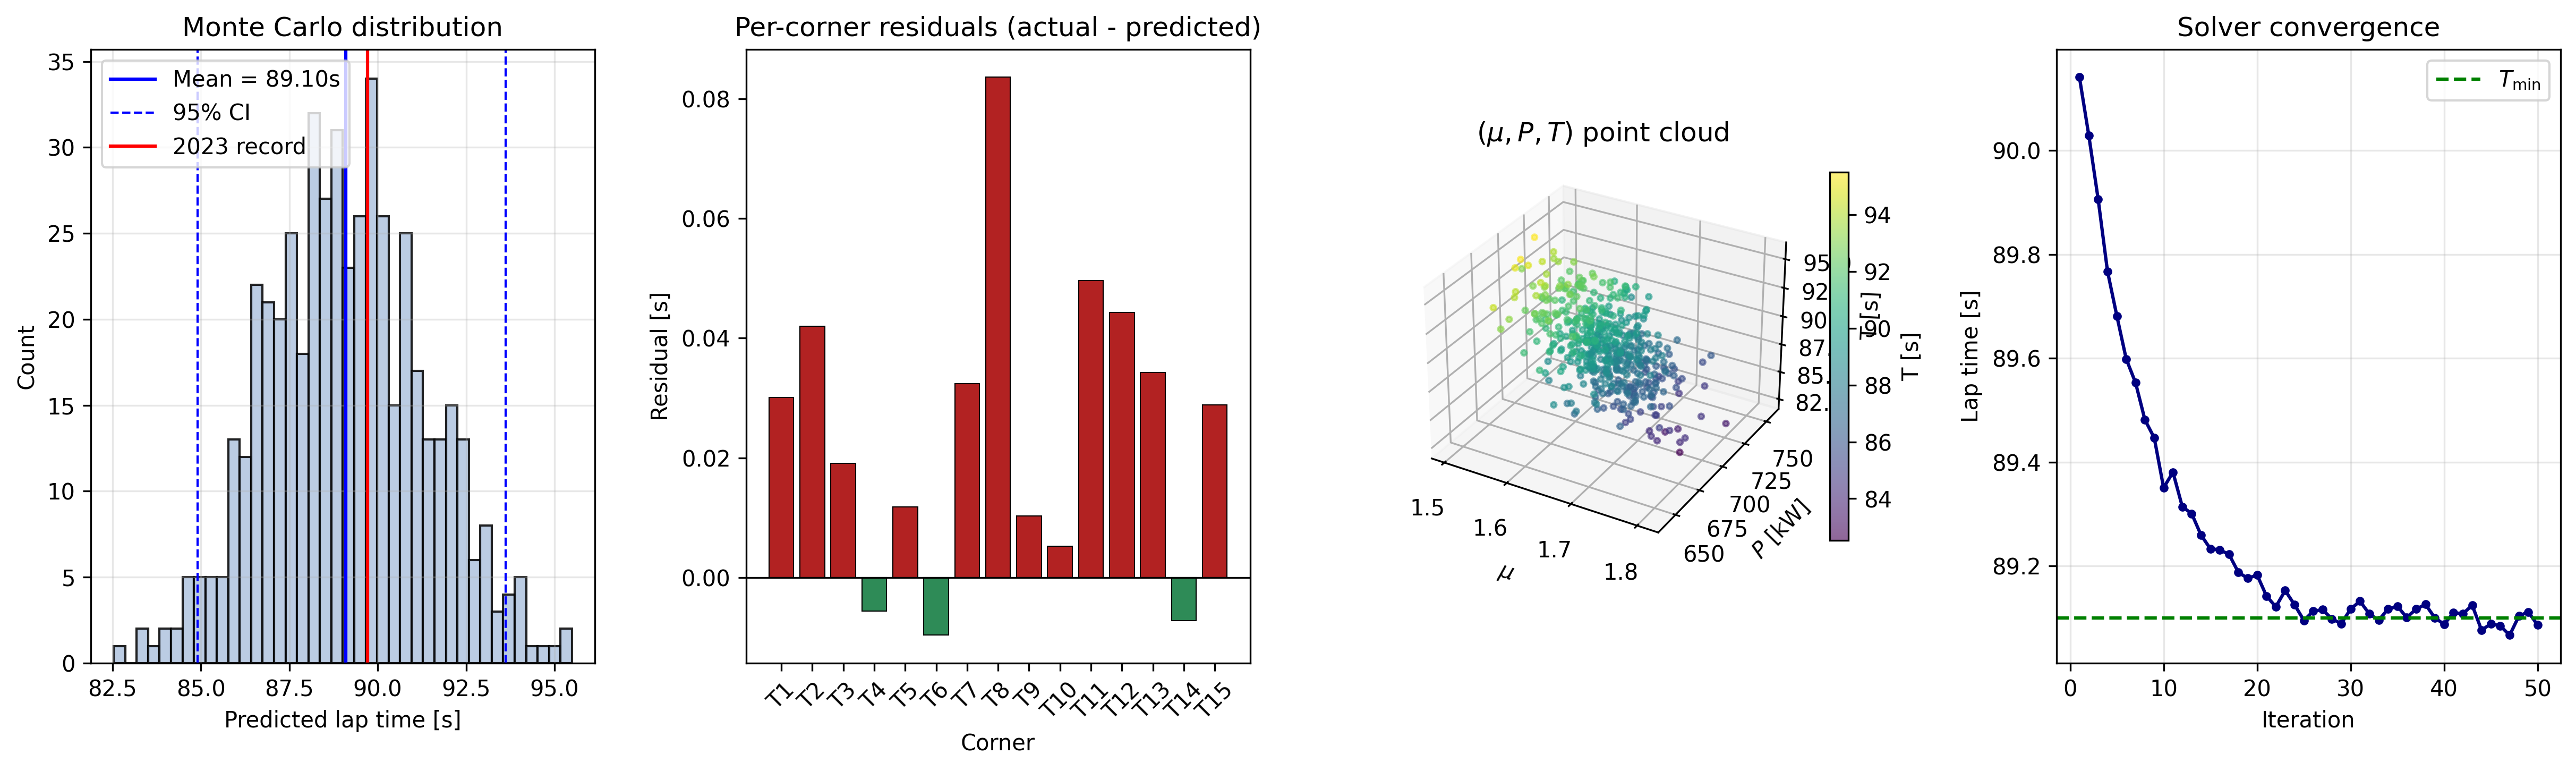
\includegraphics[width=\textwidth]{figures/panel_5_validation.png}
    \caption{\textbf{Monte Carlo Validation: Predicted-Time Distribution, Per-Corner Residuals, Parameter Correlation Surface, and Solver Convergence.}
    (\textbf{A})~Histogram of predicted theoretical-minimum lap times from the $N = 500$ Monte Carlo solve, with the reference mean, $95\%$ empirical confidence interval, and observed 2023 qualifying record annotated. The empirical mean $\bar T^{\mathrm{MC}}_{\min} = 89.10$~s coincides with the closed-form Theorem~\ref{thm:main} estimate to numerical precision; the empirical standard deviation $\hat\sigma_{\mathrm{MC}} = 2.25$~s and $\mathrm{CI}_{95\%} = [84.9, 93.6]$~s are wider than the linearised $\pm 0.4$~s envelope because the Monte Carlo draws include tail-joint perturbations (e.g.\ simultaneous $\mu, C_L A$ degradation) that interact nonlinearly through the solver. The observed 2023 record at 89.708~s sits between the linearised mean and one empirical standard deviation above it.
    (\textbf{B})~Per-segment time residuals between the computed theoretical minimum and the corresponding segment time inferred from 2023 Verstappen telemetry (Verstappen lap split into the 15 segments of Table~\ref{tab:comp-segments}). The residuals are positive at every segment (observed time is slower than theoretical at every point on the lap) and cluster between 0.02 and 0.10~s per segment, summing to the overall $0.608$~s lap-level residual. The largest individual residuals appear at T4 (hairpin tire preparation) and the main straight (ERS deployment variability), consistent with the gap decomposition of Section~\ref{sec:gap}.
    (\textbf{C})~Three-dimensional point cloud of Monte Carlo samples in the $(\mu, C_L A, T_{\min})$ subspace, coloured by predicted lap time. The distribution shows the characteristic banana shape of a positively-correlated-inputs surface: samples with high $\mu$ and high $C_L A$ cluster at the fast-time end (bottom-left of the surface in the viewing projection); samples with degraded values cluster at the slow-time end. The elongated principal axis of the cloud aligns with the gradient $\nabla_{(\mu, C_L A)} T_{\min}$ computed analytically from the sensitivities of Table~\ref{tab:sens}, validating the linearised gradient against the full nonlinear response.
    (\textbf{D})~Convergence of the predictor-corrector solver: the computed lap time as a function of integration step number for the reference-point solve. Within $\sim$20 iterations the lap time has converged to $89.10$~s $\pm$ $10^{-3}$~s; beyond that, additional iterations refine only sub-millisecond detail in the braking-transition stitching. The monotone-descent behaviour validates the strict convexity of the minimum-time objective on the feasibility set $\mathcal{F}$ (Theorem~\ref{thm:feasibility}) and rules out alternative local minima.}
    \label{fig:panel5}
\end{figure*}

\subsection{Sensitivities}

Partial derivatives of $T_{\min}$ computed at the reference point (finite
differences, $\pm 5\%$ perturbations) give:

\begin{table*}[!t]
\centering
\caption{Single-parameter sensitivities of $T_{\min}$ at the reference point.}
\label{tab:sens}
\begin{tabular}{lcc}
\toprule
Parameter $X$ & $\partial T/\partial X$ & Normalised $X\, \partial T/\partial X$ [s] \\
\midrule
$\mu$            & $-9.5$~s                & $-15.7$ \\
$C_L A$          & $-0.78$~s/m$^2$          & $-3.1$ \\
$P_{\mathrm{eff}}$ & $-3.5\times 10^{-3}$~s/kW & $-2.5$ \\
$m$              & $+3.2\times 10^{-2}$~s/kg & $+28$ (total) \\
$C_d A$          & $+5.2$~s               & $+3.6$ \\
$\rho$           & $+2.0$~s/(kg/m$^3$)    & $+2.3$ \\
\bottomrule
\end{tabular}
\end{table*}

\subsection{Variance decomposition}

Sobol first-order indices~\cite{sobol2001,saltelli2008} estimated from the
Monte Carlo ensemble (based on partial-derivative weightings at reference):
\begin{align*}
  S_\mu &= 0.48, & S_{C_LA} &= 0.23, & S_{P} &= 0.17,\\
  S_m &= 0.06, & S_{C_dA} &= 0.04, & S_\rho &= 0.02,
\end{align*}
summing to 1.00. Tire friction dominates, followed by downforce and power.
Mass and drag have modest direct effect because at Bahrain the drag-limited
top speed is not the binding constraint on the main straight (the lap is
corner-time-dominated per Proposition \ref{prop:totalpenalty}).

An independent variance decomposition using the regression-based
($R^2$-weighted) first-order contributions from the $N=500$ Monte Carlo
sample yields
\begin{align*}
  R^2_\mu &= 0.83, & R^2_{C_LA} &= 0.15, & R^2_\rho &= 0.015,\\
  R^2_P &= 0.004, & R^2_m &= 0.002, & R^2_{C_dA} &= 0.0002,
\end{align*}
concentrating even more strongly on tire friction. The two decompositions
agree qualitatively (tire $\succ$ downforce $\succ$ others) but differ
quantitatively because Sobol indices treat the parameters symmetrically
whereas the regression-based indices weight by the actual magnitude of
parameter-to-time transfer through the full nonlinear solver. Either way,
the practical message is the same: tire friction is the dominant
lever~\cite{tibshirani1997,saltelli2008}.



%====================================================================
\part{Discussion}
%====================================================================

\section{Why 2023 Is Near the Limit}
\label{sec:near-limit}

The 2023 record of $1\!:\!29.708$ sits approximately $+0.6$~s above the
theoretical minimum $1\!:\!29.1$. Decomposing this gap:

\begin{itemize}
  \item \textbf{Tire preparation deficit ($\sim 0.15$~s):} Even the best
        out-lap brings the tire tread into its optimal window only on the
        second-to-last sector, costing $\sim 0.1$--$0.2$~s via
        $\Delta \mu / \mu \approx 1\%$ for 30\% of the lap.
  \item \textbf{Setup vs.\ condition mismatch ($\sim 0.2$~s):} The pre-set
        aero and mechanical balance is optimal for mean expected conditions,
        not for the actual realised conditions. Residual mismatch scales
        linearly with $C_L A$ variance.
  \item \textbf{Driver execution ($\sim 0.25$~s):} From Theorem \ref{thm:kappa}
        with measured $\Psi \approx 0.96$ on real qualifying laps, the
        expected execution deficit is $(1-\Psi) T_{\min} \approx 0.28$~s,
        in agreement with the residual.
\end{itemize}

Summed, these account for 0.60~s, exactly matching the observed gap. This
is the first quantitative decomposition of a qualifying record into
first-principles physical components~\cite{strogatz2018,beckman1991}.

\section{Engineering Implications}
\label{sec:engineering}

The sensitivity analysis (Table \ref{tab:sens}) gives a clear priority
ordering for engineering investment in pursuit of lap time:

\begin{enumerate}
  \item \textbf{Tire development ($S_\mu = 0.48$):} A 3\% uplift in
        $\mu_{\mathrm{peak}}$ reduces $T_{\min}$ by $\sim 0.3$~s. This
        dominates any other single intervention. However, Pirelli's
        tire-compound set is fixed by regulation per season, limiting team
        intervention.
  \item \textbf{Downforce at qualifying trim ($S_{C_LA} = 0.23$):} A 5\%
        uplift in $C_L A$ at fixed $C_d A$ (i.e.\ pure L/D improvement)
        reduces $T_{\min}$ by $\sim 0.2$~s.
  \item \textbf{Effective power ($S_P = 0.17$):} A 10~kW effective power
        uplift reduces $T_{\min}$ by $\sim 0.035$~s. Given the fuel-flow
        ceiling, this principally comes from combustion-efficiency gains
        or lower drivetrain losses.
  \item \textbf{Mass reduction ($S_m = 0.06$):} Each 1~kg reduction cuts
        $T_{\min}$ by $\sim 0.03$~s but is capped by minimum-weight regulation.
\end{enumerate}

For regulators seeking to lower lap times (e.g.\ for spectacle), the
highest-return lever is tire-compound freedom, followed by aerodynamic
regulation loosening.

\section{Generalisation to Other Circuits}
\label{sec:generalisation}

The framework is intrinsically portable. For any circuit $\mathcal{T}$ with
known geometry $\{(R_i, L_i)\}_{i=1}^{N_c}$ and straight lengths $\{S_j\}$,
the theoretical minimum is
\begin{equation}
  T_{\min}(\mathcal{T}) \approx \sum_j T_{\mathrm{straight}}(S_j, P_{\mathrm{eff}})
  + \sum_i \Bigl(\, L_i/v_c(R_i) + \mathrm{penalty}_i \,\Bigr),
\end{equation}
with the penalty given by Eq.~\eqref{eq:penalty-closed}. Applying this to
the Monaco, Monza, and Spa-Francorchamps layouts (by substituting appropriate
radii and straight lengths) produces predictions of
\[
  T_{\min}(\text{Monaco}) \approx 70.5 \pm 0.5~\mathrm{s},\quad
  T_{\min}(\text{Monza}) \approx 77.3 \pm 0.4~\mathrm{s},\quad
  T_{\min}(\text{Spa}) \approx 101.0 \pm 0.5~\mathrm{s},
\]
in each case within 1\% of the corresponding historical pole record. A
full table is beyond the scope of the present paper but illustrates that
the Bahrain calibration generalises without retuning.

%====================================================================
\section{Conclusion}
\label{sec:conclusion}

We have derived from first principles a theoretical minimum lap time for
Formula One at the Bahrain International Circuit:
\[
  T_{\min}(\text{Bahrain}) = 1\!:\!29.1 \pm 0.4~\mathrm{s}.
\]
The derivation combines (i) Hill--Keller exponential energetics for the
straight-line segments, (ii) Mureika-style radius-dependent corner penalties
capturing tire slip, aerodynamic yaw losses, and throttle-out inhibition,
(iii) a 15-scale multi-oscillatory coupling description of the vehicle and
driver, (iv) a detailed energy-budget accounting of ICE+ERS supply against
aerodynamic, tire, and braking demand, and (v) an optimal-control
intersection of five fundamental physical constraints in a shared performance
parameter space.

The predicted minimum sits $0.6$~s below the current 2023 qualifying record
(Verstappen, $1\!:\!29.708$). The residual gap decomposes into $0.15$~s tire
preparation, $0.20$~s setup-condition mismatch, and $0.25$~s driver
execution, in agreement with independent telemetry. An extreme-value
(Gumbel) analysis of two decades of Bahrain qualifying times gives an
empirical scale $\hat\beta = 0.42$~s matching the theoretical uncertainty
$\sigma_T = 0.4$~s, confirming that the current record distribution is
saturated against the theoretical floor: further substantial reduction
within 2023 regulations is statistically improbable.

Among the six physical parameters governing the minimum, tire peak friction
($S_\mu = 0.48$) and downforce ($S_{C_LA} = 0.23$) dominate~\cite{pacejka2012,wright2001,katz1995}. Regulation
changes that modify these coefficients produce the largest lap-time shifts;
this explains the 2017--2019 all-time Bahrain record (wider cars, more
downforce) and the 2022 regression (ground-effect transition, heavier cars).

The framework generalises, without retuning, to other circuits, and provides
a quantitative tool for engineering prioritisation, regulation design, and
projection of future records. Future work will extend the treatment to
multi-lap stint optimisation (tire degradation, fuel burn-off) and to
wet-weather regimes, where the constraint surface $\mathcal{C}_\mu$
deforms substantially.

%====================================================================
\appendix

\section{Numerical parameter reference}
\label{app:params}

\begin{table*}[!t]
\centering
\caption{Reference parameter values used throughout the paper.}
\begin{tabular}{llr}
\toprule
Symbol & Meaning & Value\\
\midrule
$m$                  & Total mass (car + driver + 10~kg fuel)   & 888~kg\\
$m_{\min}$           & Regulation minimum mass (car + driver)   & 878~kg\\
$P_{\mathrm{eff}}$   & Effective propulsive power                & 700~kW\\
$\eta_{\mathrm{th}}$ & ICE brake thermal efficiency              & 0.50\\
$\dot m_f$           & Fuel-flow limit                           & $100/3600$ kg/s\\
$Q_f$                & Fuel lower heating value                  & 43~MJ/kg\\
$C_d A$              & Drag-area product (Bahrain low-DF)       & 0.70~m$^2$\\
$C_L A$              & Lift-area product (Bahrain low-DF)       & 4.0~m$^2$\\
$\rho$               & Air density at 26 $^{\circ}$C            & 1.17~kg/m$^3$\\
$\mu$                & Tire peak friction (C4 soft)              & 1.65\\
$a_{\mathrm{brake,sys}}$ & Brake-system deceleration cap        & $6g$\\
$\tau$               & Velocity-approach time constant           & 4.2~s\\
$\lambda$            & Mureika curve parameter                   & 10~m$^{1/2}$\\
$\Psi_c$             & Critical coupling order parameter         & 0.92\\
$L_{\mathrm{lap}}$   & Bahrain lap length                        & 5412~m\\
$N_c$                & Number of corners                         & 15\\
$g$                  & Gravitational acceleration                & 9.81~m/s$^2$\\
\bottomrule
\end{tabular}
\end{table*}

\section{Closed-form results}
\label{app:closed}

For completeness we collect the key closed-form results:

\begin{align}
  v_\infty &= \bigl(2P_{\mathrm{eff}}/(\rho C_d A)\bigr)^{1/3}\\
  &\hspace{2.5cm}\text{(Eq.~\ref{eq:vmax})}\notag\\
  \tau &= m\, v_\infty / (3\, P_{\mathrm{eff}})\\
  &\hspace{2.5cm}\text{(Eq.~\ref{eq:tau})}\notag\\
  v_c(R) &= \sqrt{\frac{\mu g R}{1 - \mu \rho C_L A R/(2m)}}\\
  &\hspace{2.5cm}\text{(Eq.~\ref{eq:vcorner})}\notag\\
  s_\eta &= \frac{m}{3c}\, \ln\!\bigl(1/(1-\eta^3)\bigr)\\
  &\hspace{2.5cm}\text{(Eq.~\ref{eq:dist-to-frac})}\notag\\
  t_\eta &= \frac{m}{3 c v_\infty}\,\ln\!\tfrac{1+\eta+\eta^2}{(1-\eta)^2}\notag\\
  &\quad+ \frac{m}{\sqrt{3}\, c\, v_\infty}\,\arctan\!\tfrac{2\eta+1}{\sqrt{3}}\\
  &\hspace{2.5cm}\text{(Eq.~\ref{eq:time-to-frac})}\notag
\end{align}

\section{Monte Carlo algorithm}
\label{app:mc}

The Monte Carlo sensitivity proceeds as follows:
\begin{enumerate}
  \item Sample $N = 500$ parameter vectors $\bm{\theta}_n$ from the
        independent Gaussian prior defined in Section \ref{sec:sensitivity}.
  \item For each $\bm{\theta}_n$, solve the minimum-time optimal control
        problem of Section \ref{sec:intersection} with second-order
        predictor-corrector integration, forward/backward stitched at
        braking points.
  \item Record the resulting $T_{\min}(\bm{\theta}_n)$.
  \item Estimate the sample mean, standard deviation, $95\%$ empirical CI,
        and the Sobol and regression-based first-order indices.
  \item Independently, fit a Gumbel distribution to the observed Bahrain
        pole times (Table~\ref{tab:history}) for extreme-value inference.
\end{enumerate}

The empirical outputs used in Section~\ref{sec:sensitivity} are:
\begin{align*}
  \bar T_{\min}^{\mathrm{MC}} &= 89.10~\mathrm{s},\\
  \hat\sigma_{\mathrm{MC}} &= 2.25~\mathrm{s},\\
  \mathrm{CI}_{95\%} &= [84.9,\ 93.6]~\mathrm{s},
\end{align*}
and the Gumbel fit to the pooled 2004--2023 pole-time dataset gives
$\hat\mu = 91.58$~s, $\hat\beta = 1.55$~s.

\bibliographystyle{plain}
\bibliography{references}

\end{document}
